\documentclass{article}
\usepackage[utf8]{inputenc}
\usepackage[english]{babel}
\usepackage[normalem]{ulem}
\usepackage{amssymb}
\usepackage{amsmath}
\usepackage{graphicx}
\usepackage{algorithm}
\usepackage{algorithmic}
\title{Rapport sur le projet d'Optimisation\\Support-Vector Machines}
\author{Kawisorn Kamtue \& Clémence Réda}
\date{\today}

\begin{document}

\maketitle

\section{Support Vector Machine}

Les \emph{Support Vector Machine solvers} (SVM) sont une catégorie d'algorithmes d'apprentissage statistique supervisé. Ils permettent de résoudre le problème de classification binaire suivant :\\

           
           Etant donnés $(x_i)_{i \leq m}$ des points dans $\mathbb{R}^n$, et $(y_i)_{i \leq m}$ les étiquettes des points tels que l'étiquette de $x_i$ soit $y_i \in \{-1, 1\}$, on cherche la droite qui sépare "le mieux possible" les points dans différentes classes, autrement dit, la frontière de Voronoi entre les deux classes.
           \begin{center}
           \begin{figure}[H]
           \centering
           \caption{Exemple de frontière pour deux classes : celles des points bleus et celle des points rouges}
           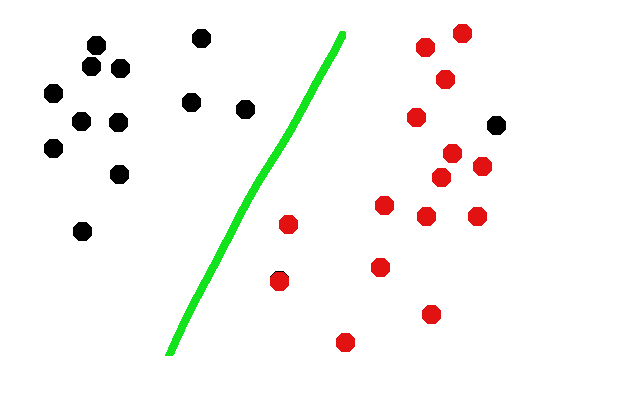
\includegraphics[scale=0.3]{images/voronoi.png}
           \end{figure}
           \end{center} 

\noindent La frontière que l'on recherche est une fonction linéaire, donc de la forme (avec deux paramètres de dimension 1 $\omega$ et $b$) :\\

          \begin{center}
          $f : X \rightarrow \omega^{T}X + b = $ \begin{bmatrix} $\omega$ & $b$ \end{bmatrix} \begin{bmatrix} $x$\\ 1 \end{bmatrix}
          \end{center}

telle que :\\
 
         \begin{center}
         $\forall i, y_i = -1 \Rightarrow f(x_i) \leq -1$\\
         $\forall i, y_i = 1 \Rightarrow f(x_i) \geq 1$\\
         $\Leftrightarrow \forall i, y_i \times f(x_i) \geq 1$ (1)
         \end{center}

Pour simplifier le problème, on peut prendre $ \omega' = $ \begin{bmatrix}$ \omega$\\ $b$\end{bmatrix} et $x' =$\begin{bmatrix}$x$\\ 1\end{bmatrix} (que l'on notera par souci de simplicité $\omega$ et $x$).\\

Pour obtenir un résultat robuste, on souhaite que les deux droites $f(X) = 1$ et $f(X) = -1$ soient les plus distantes possibles. En effet, si ces deux droites sont trop proches, cela signifie que la probabilité d'erreur quant à la prédiction de la classe d'un point proche de ces droites sera importante.\\

La distance $\gamma$ entre ces deux droites se calcule de la façon suivante : soient $u, v$ deux points tels que $f(v) = 1$ et $f(u) = -1$. Alors :

      \begin{center}
      $\|f(v) - f(u)\| = \|\omega \times (v-u)\| = \|\omega\| \times \|(v-u)\| = \|\omega\| \times \|\gamma\| = \|1 - (-1)\| = 2$
      \end{center}

Finalement, le problème d'optimisation à résoudre pourrait être :\\
 
           \begin{center}
           $max_{w}$ $\gamma = \frac{2}{\|w\|}$ avec (1)\\
           $\Leftrightarrow min_{w}$ $\|w\|$ avec (1)\\
           $\Leftrightarrow min_{w}$ $\frac{1}{2} \times \|w\|^2$ avec (1) pour faciliter les calculs
           \end{center}

\bigskip

Un autre problème se pose si on s'arrête ici : par exemple, dans l'exemple de la frontière de Voronoi que l'on a vu ci-dessus, si on a un point bleu au milieu des points rouges, alors il n'existe pas de droite telle qu'il n'y ait que de points bleus d'un côté et que des points rouges de l'autre côté, ce qui contredit la condition (1). Le problème est alors infaisable. Pourtant, la droite dessinée en vert peut sembler acceptable comme frontière pour l'ensemble de points auquel on a ajouté un point bleu au milieu du nuage de points rouge.\\

On tient compte de cette erreur en introduisant les variables $(z_i)_{i \leq m}$. Pour que la condition (1) soit toujours vérifiée, il faut que quand $y_i \times f(x_i) \geq 1$, $z_i = 0$ et lorsque $y_i \times f(x_i) < 1$, $z_i = 1 - y_i \times f(x_i)$. Le but étant de minimiser le nombre de ces erreurs, ie. points mal classés, on utilise un paramètre $C$ constant qui permet d'insister plus ou mins sur la minimisation de ces erreurs :\\ 


           \begin{center}
           (P) $min_{w}$ $\frac{1}{2} \times \|w\| + C \times \sum_{i \leq m}z_i$\\
           avec $\forall i, z_i \geq 0$\\
           $\forall i, y_i \times (\omega^{T} x_i) \geq 1 - z_i$\\
           \end{center}

\bigskip

Les fonctions que l'on a introduites sont toutes convexes. Si la dimension des points $(x_i)_i$ est petite, nous allons pouvoir utiliser la méthode de Newton pour résoudre ce problème. On verra par la suite le \emph{kernel trick} qui permettra de ne pas tenir compte de la dimension, mais seulement du nombre d'échantillons $(x_i)_i$.

\section{Calcul du dual}

Calculons le lagrangien du problème (P). Soit $\lambda$ le multiplicateur de Lagrange de dimension $1 \times m$:

              \begin{center}
              $\forall w, \lambda \in \mathbb{R}^{2m}, L(\omega, \lambda, z) = $\\
              $= \frac{1}{2} \|w\|^2 + C \times \sum_i z_i - \sum_i \lambda_i \times z_i$
              $+ \sum_i \lambda_i \times (1 - y_i \omega^{T} x_i)$\\
              $= \frac{1}{2} \|w\|^2 + C$\textbf{1}$^{T}z - C\lambda^{T}z + $\textbf{1}$^{T}\lambda - \sum_i \lambda_i \times y_i \omega^{T} x_i$\\
              $= \frac{1}{2} (\|w - \sum_i \lambda_iy_ix_i\|^2_2 - \|\sum_i \lambda_iy_ix_i\|^2_2)$
              $+ (C$\textbf{1}$ - \lambda)^{T}z + $\textbf{1}$^{T}\lambda$\\
              \end{center}

Minimisons L par rapport à $\omega$. Comme le lagrangien est convexe en $\omega$, il faut annuler le gradient :\\

              \begin{center}
              $\nabla_{\omega} L(\omega, \lambda, z) = \frac{1}{2}(2\omega - 2\sum_i \lambda_iy_ix_i) + 0 = 0$\\
              $\Leftrightarrow \omega = \sum_i \lambda_iy_ix_i$ (1)\\
              \end{center}

Minimisons L par rapport à $z$. Comme le lagrangien est convexe en $z$, il faut annuler le gradient :\\

              \begin{center}
              $\nabla_{z} L(\omega, \lambda, z) = 0 + C$\textbf{1}\textbf{$1_{z>0}$}$^T - \lambda$\textbf{$1_{z>0}$}$^T = 0$\\
              $\Leftrightarrow mC - \sum_i \lambda_i = 0$ si $z_i > 0$\\
              $\Leftrightarrow mC = \sum_i \lambda_i$ si $z_i > 0$\\
              \end{center}

Le minimum en L par rapport à $z$ a une valeur finie ssi $C$\textbf{1}$ - \lambda = 0$. On obtient le problème dual en injectant les valeurs de $\omega$ et de $z$ dans le lagrangien :\\

             \begin{center}
             $max_{\lambda \in \mathbb{R}^{+m}} -\frac{1}{2}\|\sum_i\lambda_iy_ix_i\|^2_2 + $\textbf{1}$^T\lambda$ par (1)\\ 
             avec $\forall i, 0 \leq \lambda_i \leq C$ si $z_i > 0$\\
            (vient des conditions de KKT -\emph{complementary slackness},\\
            vérifiées car le problème est convexe)\\
             \end{center}

On obtient la solution optimale du primal $(\omega^*, z^*)$ à partir de celle du dual $\lambda^*$ :

             \begin{center}
             (1) $\omega^{*} = \sum_i \lambda^{*}_i y_i x_i$
             \end{center}

\section{Utilisation de l'astuce du noyau (\emph{kernel trick})}

Pour pouvoir trouver efficacement la solution au problème avec la méthode de Newton, il faut s'affranchir de la contrainte quadratique sur la dimension des échantillons. On note X la matrice des échantillons, et la matrice du noyau $K = X^TX$, avec $K \geq 0$. On montre alors que le problème dual peut se réécrire de la façon suivante :\\

                 \begin{center}
                 $max$ $-\frac{1}{2}\lambda^Tdiag(y)Kdiag(y)\lambda+$\textbf{1}$^T\lambda$\\
                 avec $\forall i, 0 \leq \lambda_i \leq C$ 
                 \end{center}

ce qui équivalent à :\\

            \begin{center}
                 $min$ $\frac{1}{2}\lambda^Tdiag(y)Kdiag(y)\lambda-$\textbf{1}$^T\lambda$\\
                 avec $\forall i, 0 \leq \lambda_i \leq C$ 
                 \end{center}

On remarque que la dimension $m$ des échantillons n'intervient plus, et que donc la complexité de la résolution du problème ne dépend que du nombre d'échantillons. 

\section{Méthode de la barrière logarithmique}

Enfin, on peut s'affranchir des contraintes d'inégalité sur le multiplicateur de Lagrange $\lambda$ en posant la fonction barière suivante :\\

          \begin{center}
          $\Phi(\lambda) = \sum_i (- log(C - \lambda_i) - log(\lambda_i)) = \sum_i log(\frac{1}{(C - \lambda_i)\lambda_i}) = - \sum_i log((C - \lambda_i)\lambda_i)$ 
          \end{center}

Cette fontion vaut $+\infty$ si $a<0$ ou $a>C$.Le problème à optimiser devient alors (en changeant le signe pour obtenir une fonction à minimiser) :\\

          \begin{center}
                 $min$ $\frac{1}{2}\lambda^Tdiag(y)Kdiag(y)\lambda-$\textbf{1}$^T\lambda +\Phi(\lambda)$\\
                 avec $\forall i, 0 \leq \lambda_i \leq C$ 
                 \end{center}
\section{Résultats}

\subsection{Comparaison entre les différentes générations de points}

\subsubsection{Tableau récapitulatif}

$d$ est la dimension des points et $n$ le nombre d'échantillons dans la génération. On utilise $\frac{2}{3}$ des points (choisis au hasard uniformément) de l'ensemble de départ pour l'ensemble d'entraînement, et les points restants pour l'ensemble de validation. \\

     \begin{table}[H]
       \caption{Comparaison entre les générations de points}
       \begin{tabular}{|l|c|c|c|c|c|c|r|}
         \hline
         \textsc{Données} & \textsc{C} & \textsc{d} & \textsc{n} & \textsc{N it.} & \textsc{Temps (s)} & \textsc{Meilleur C} & \textsc{Echec (\%)}\\
         \hline
         1 & 1 & 40 & 10 & 11 & 25,414 & 1 & 0 (*)\\
         \hline
         1 & 5 & 40 & 10 & 11 & 0,177 & 1 & 0 (*)\\
         \hline
         1 & 10 & 40 & 10 & 11 & 0,168 & 1 & 0 (*)\\
         \hline
         1 & 5 & 40000 & 10 & 11 & 0,315 & X & 0\\
         \hline
         1 & 5 & 40 & 100 & 12 & 0,715 & X & 0\\
         \hline
         1 & 5 & 40 & 1000 & ? & > 10 & ? & ?\\
         \hline
         2 & 5 & 200 & 150 & 12 & 0,689 & ? & 0\\
         \hline
         3 & 5 & 200 & 150 & 12 & 0,660 & ? & 0\\
         \hline
         4 & 5 & 200 & 150 & 12 & 0,655 & ? & 0\\
         \hline
         5 & 5 & 200 & 150 & 12 & 0,709 & ? & 4\\
         \hline
       \end{tabular}
     \end{table}

Quelques remarques :
\begin{itemize}
\item De manière générale, utiliser une valeur de C plus grande accélère considérablement la recherche de la solution duale : pas au niveau du nombre d'itérations de la méthode de Newton, mais au niveau du coût de l'appel à la méthode de Newton (voir les trois premiers tests). 
\item La complexité temporelle de la résolution du problème dual est bien indépendante de la dimension et dépendante de la taille de l'échantillon (voir les tests 4, 5 et 6).
\item La valeur "?" signifie que l'algorithme a tourné trop longtemps pour la valeur soit mesurée.
\item La notation "(*)" signifie que les tests marqués ont utilisé le même ensemble de données.
\end{itemize}

\subsubsection{Validation croisée pour le choix de la meilleure valeur de $C$}

Les deux fonctions \emph{choiceC} et \emph{crossvalidation} permettent de sélectionner la meilleure valeur de C pour un échantillon donné, par la méthode de \emph{leave-one-out}, où, pour un échantillon de taille $n$, à chaque itération on choisit un élément $e$ comme ensemble de test, et l'entraînement du SVM se fait sur les $n-1$ éléments restants. La valeur de C qui permet d'obtenir une erreur globale (sur l'ensemble d'itérations) minimale est considérée la meilleure.

\subsection{Points dans les quadrants ($x, y > 0$) et ($x > 0, y < 0$)}

On génère les points selon la procédure $m = 2$ dans \emph{generatedata.m}. Les points de la première classe sont dans le quadran ($x, y > 0$) et ceux de la seconde classe sont dans le quadran ($x > 0, y > 0$). Voir le fichier \emph{test1.mat} dans le dossier \emph{test}. La meilleure valeur, au niveau du nombre d'erreurs, de $C$, choisie par validation croisée dans l'intervalle [1, 10], est 1 (les autres valeurs de C de 2 à 10 donnent le même nombre d'erreurs pour cet ensemble de données).

\subsubsection{Pour $C=1, n=10, d=40$}

     \begin{table}[H]
       \caption{Matrice de confusion pour l'ensemble de données 1}
       \begin{tabular}{|l|c|r|}
         \hline
         \textsc{Réalité/Prédiction} & \textsc{Classe 1} & \textsc{Classe 2}\\
         \hline
         \textsc{Classe 1} & 2 & 0\\
         \hline
         \textsc{Classe 2} & 0 & 1\\
         \hline
       \end{tabular}
     \end{table}

         \begin{figure}
           \begin{center}
             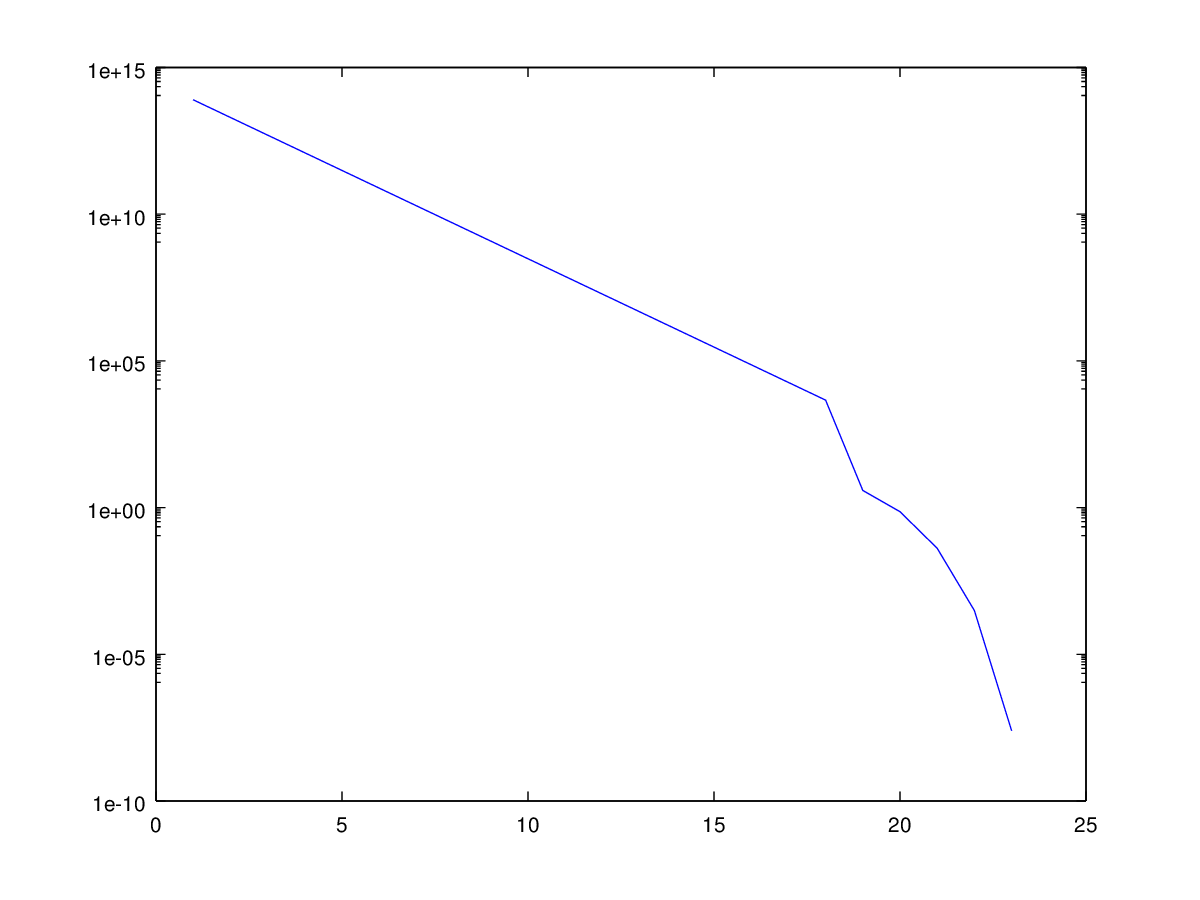
\includegraphics[scale=0.5]{images/cvnewton1.png}
             \caption{Ensemble de données 1 (échelle semi-log)}
           \end{center}
         \end{figure}

         \begin{figure}
           \begin{center}
             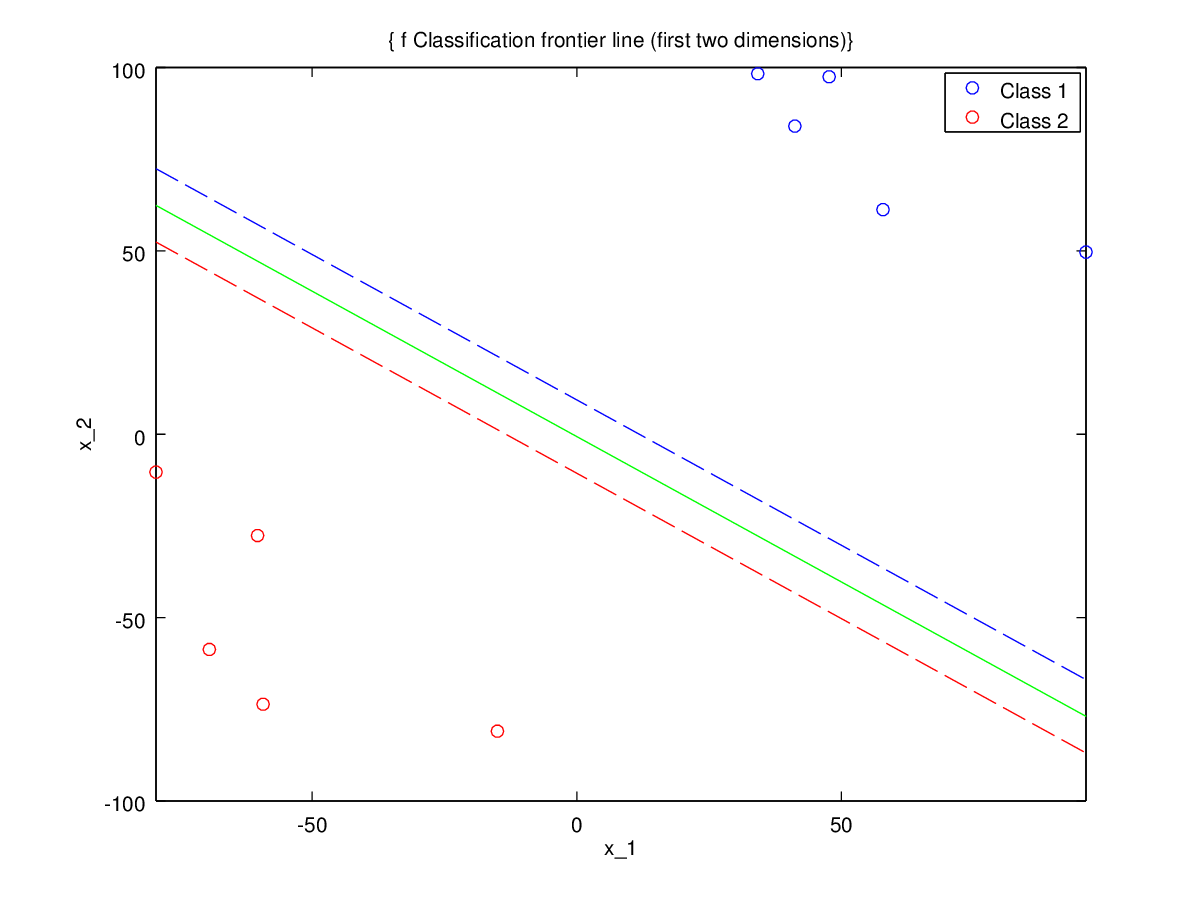
\includegraphics[scale=0.5]{images/line1.png}
             \caption{Ensemble de données 1 (Les lignes rouge et bleue en pointillés sont les droites f(x) = 10 et f(x) = -10)}
           \end{center}
         \end{figure}

         \begin{figure}
           \begin{center}
             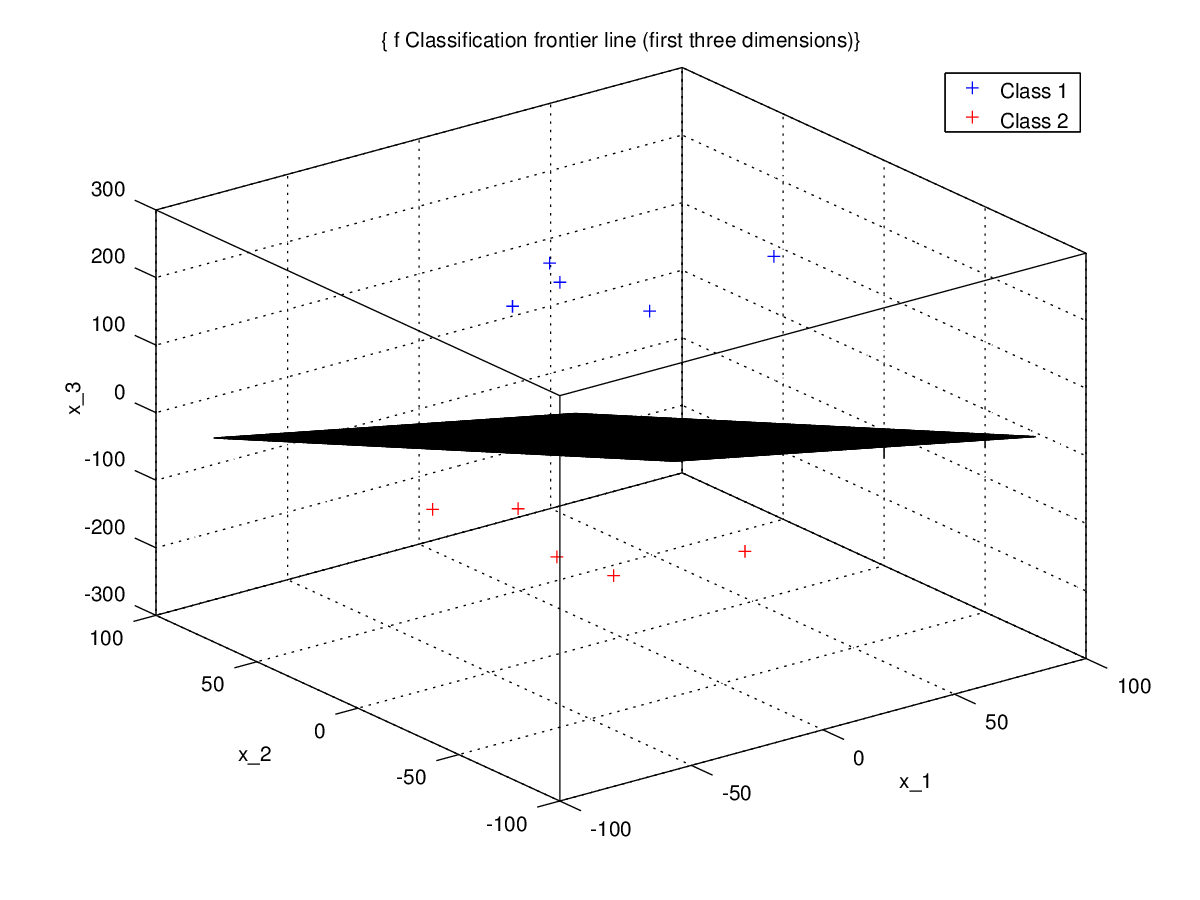
\includegraphics[scale=0.5]{images/plane1.png}
             \caption{Ensemble de données 1}
           \end{center}
         \end{figure}

         \begin{figure}
           \begin{center}
             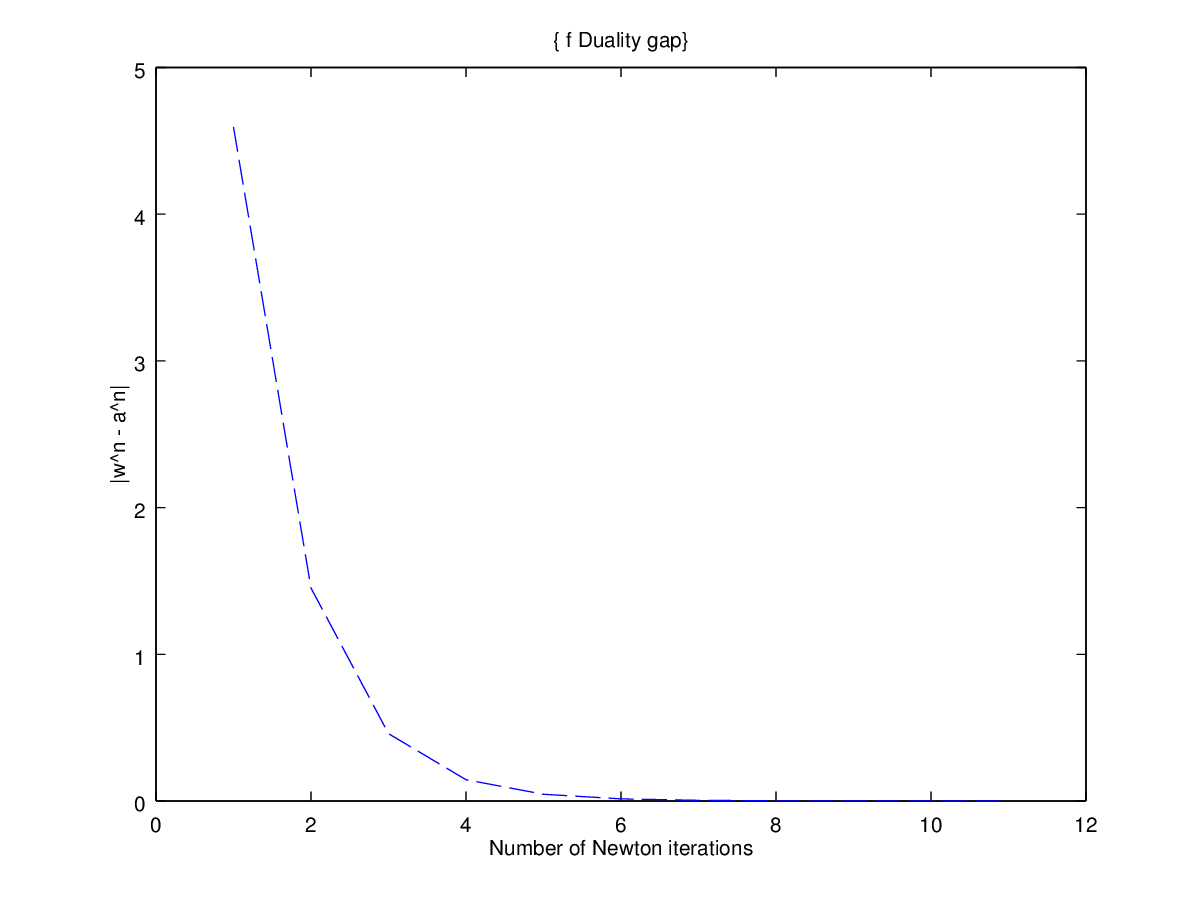
\includegraphics[scale=0.5]{images/duality1.png}
             \caption{\emph{Duality gap} : ensemble de données 1}
           \end{center}
         \end{figure}

\subsection{Points centrés réduits générés à partir de deux fonctions gaussiennes}

On génère les points selon la procédure $m = 0$ dans \emph{generatedata.m} avec $sep=10$. On tire les coordonnées en utilisant la fonction \emph{randn}, qui retourne des éléments centrés réduits générés par une Gaussienne, auxquels on retire ou ajoute 10. Voir le fichier \emph{test2.mat} dans le dossier \emph{test}. 

\subsubsection{Pour $C=5, n=150, d=200$}

     \begin{table}[H]
       \caption{Matrice de confusion pour l'ensemble de données 2}
       \begin{tabular}{|l|c|r|}
         \hline
         \textsc{Réalité/Prédiction} & \textsc{Classe 1} & \textsc{Classe 2}\\
         \hline
         \textsc{Classe 1} & 23 & 0\\
         \hline
         \textsc{Classe 2} & 0 & 27\\
         \hline
       \end{tabular}
     \end{table}

         \begin{figure}
           \begin{center}
             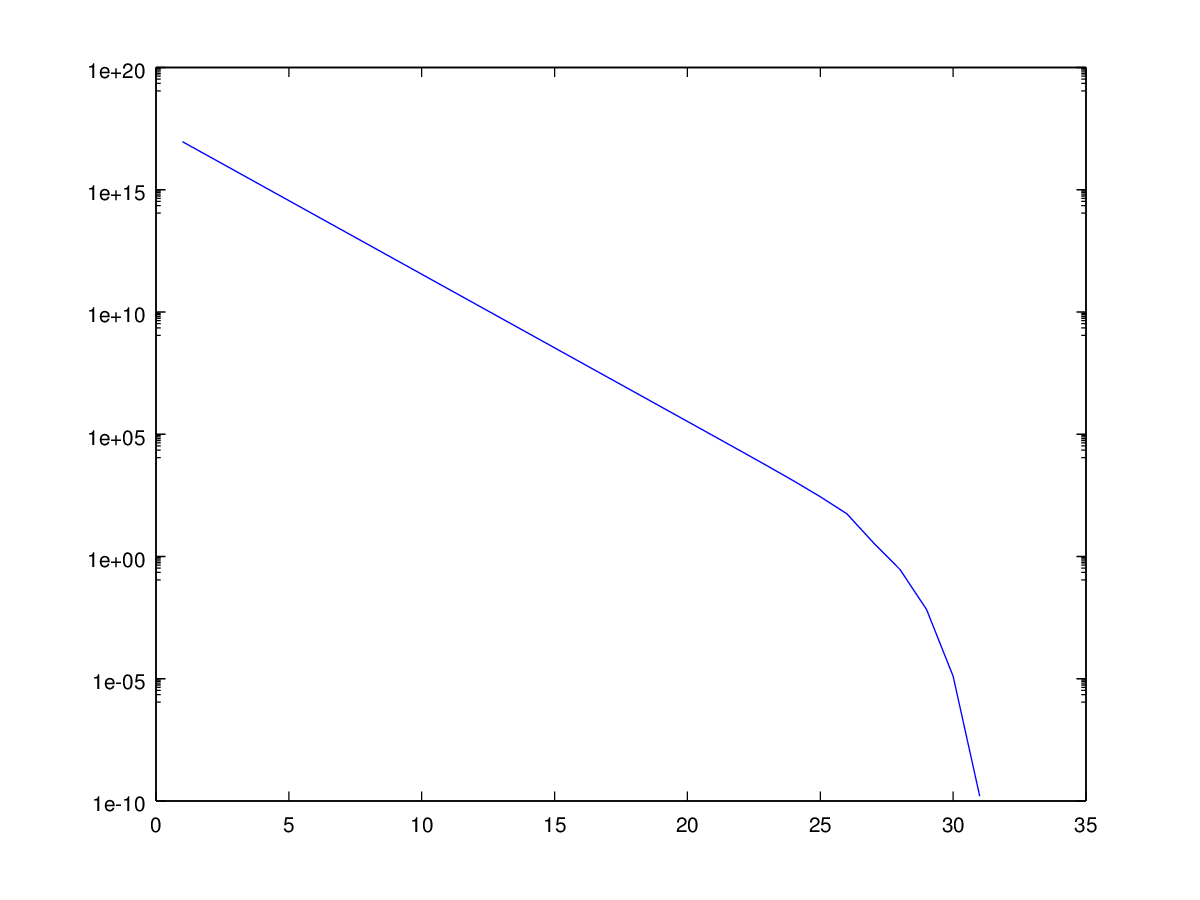
\includegraphics[scale=0.5]{images/cvnewton2.png}
             \caption{Ensemble de données 2 (échelle semi-log)}
           \end{center}
         \end{figure}

         \begin{figure}
           \begin{center}
             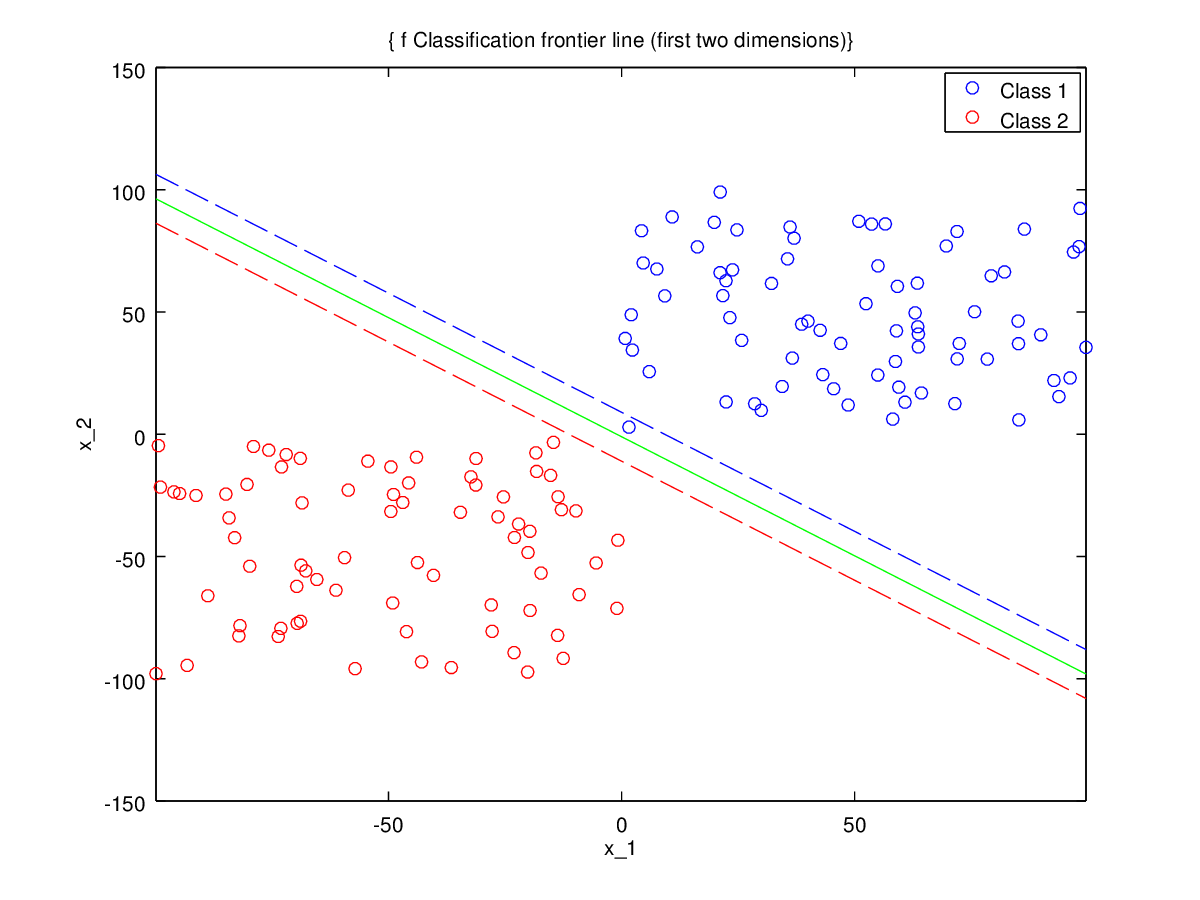
\includegraphics[scale=0.5]{images/line2.png}
             \caption{Ensemble de données 2 (Les lignes rouge et bleue en pointillés sont les droites f(x) = 10 et f(x) = -10)}
           \end{center}
         \end{figure}

         \begin{figure}
           \begin{center}
             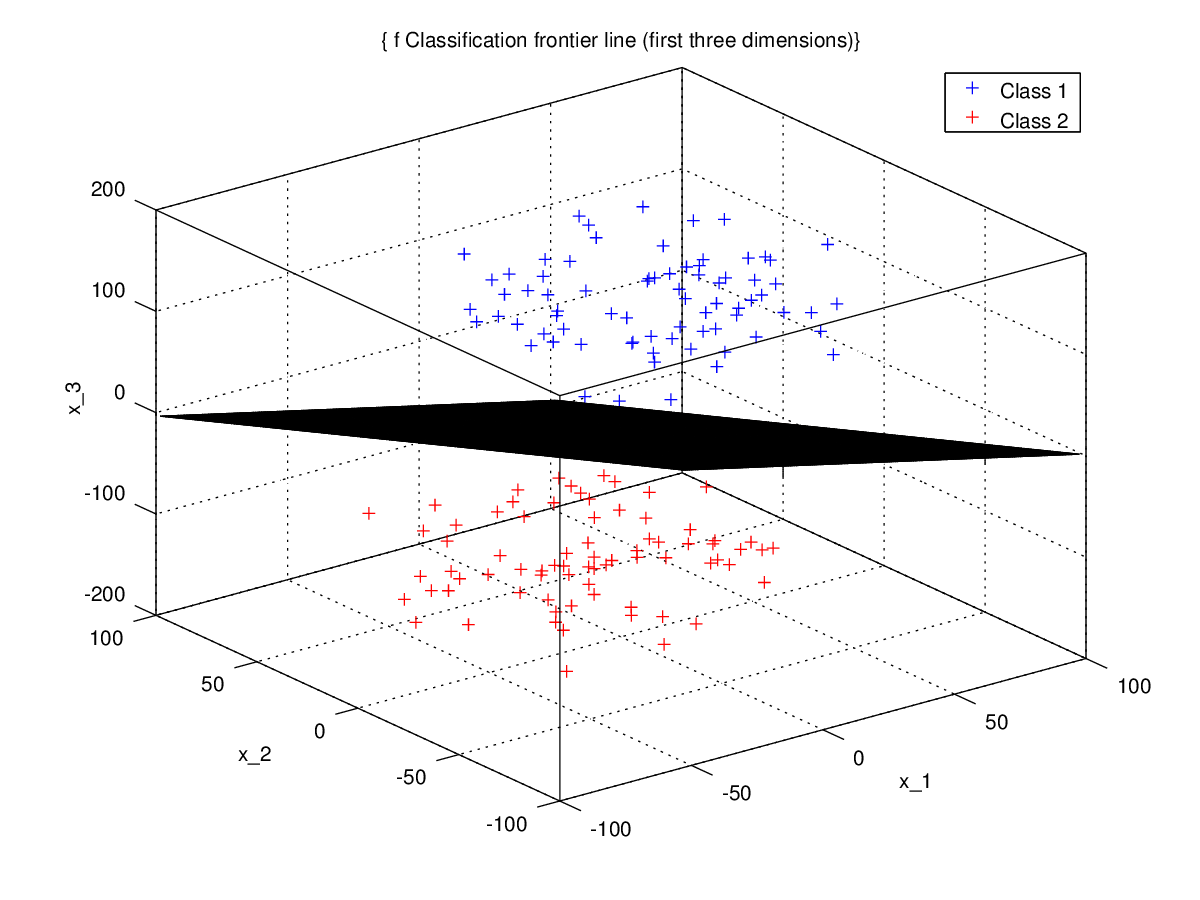
\includegraphics[scale=0.5]{images/plane2.png}
             \caption{Ensemble de données 2}
           \end{center}
         \end{figure}

         \begin{figure}
           \begin{center}
             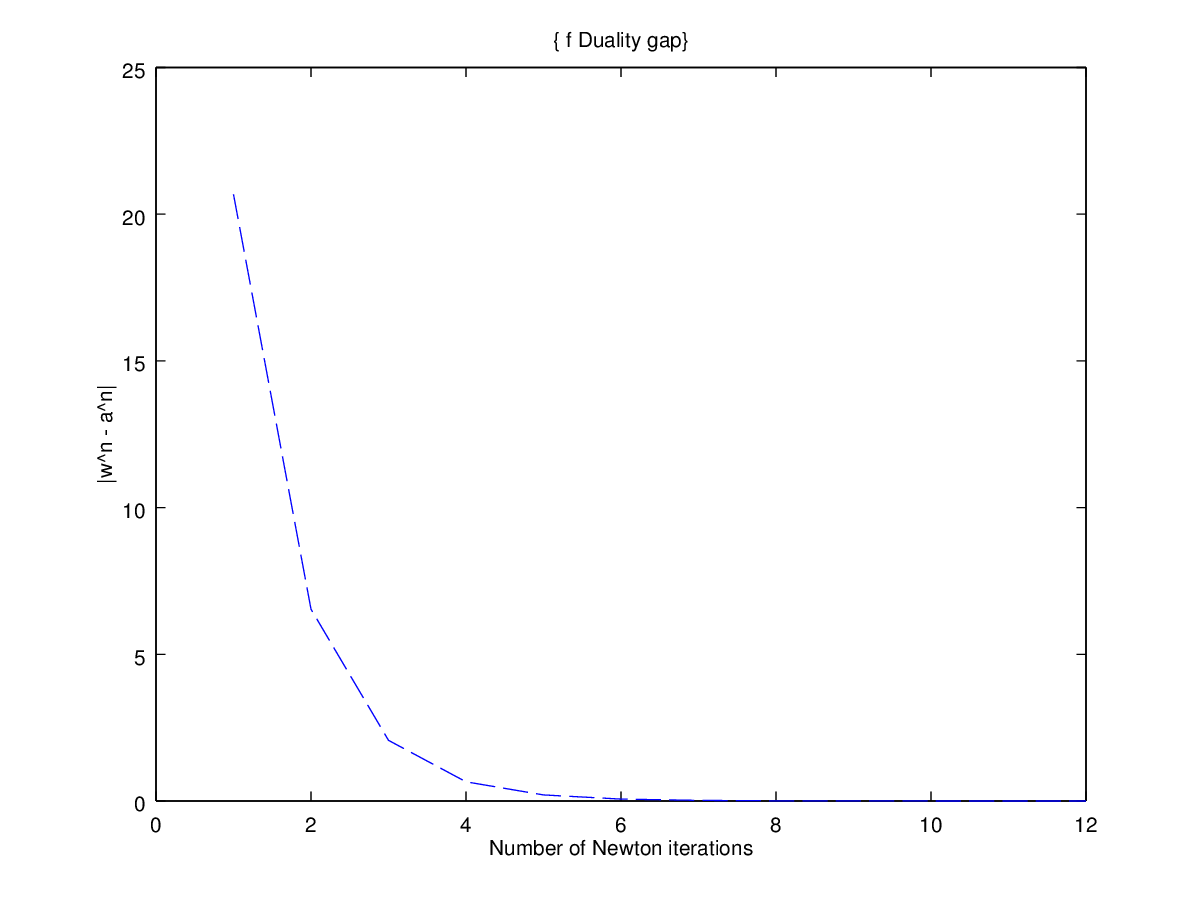
\includegraphics[scale=0.5]{images/duality2.png}
             \caption{\emph{Duality gap} : ensemble de données 2}
           \end{center}
         \end{figure}

\subsection{Points centrés réduits générés avec des fonctions gaussiennes}

On utilise la procédure $m = 0$ dans \emph{generatedata.m} avec $sep=100$. Voir le fichier \emph{test3.mat} dans le dossier \emph{test}. 

\subsubsection{Pour $C=5, n=150, d=200$}

     \begin{table}[H]
       \caption{Matrice de confusion pour l'ensemble de données 3}
       \begin{tabular}{|l|c|r|}
         \hline
         \textsc{Réalité/Prédiction} & \textsc{Classe 1} & \textsc{Classe 2}\\
         \hline
         \textsc{Classe 1} & 28 & 0\\
         \hline
         \textsc{Classe 2} & 0 & 22\\
         \hline
       \end{tabular}
     \end{table}

         \begin{figure}
           \begin{center}
             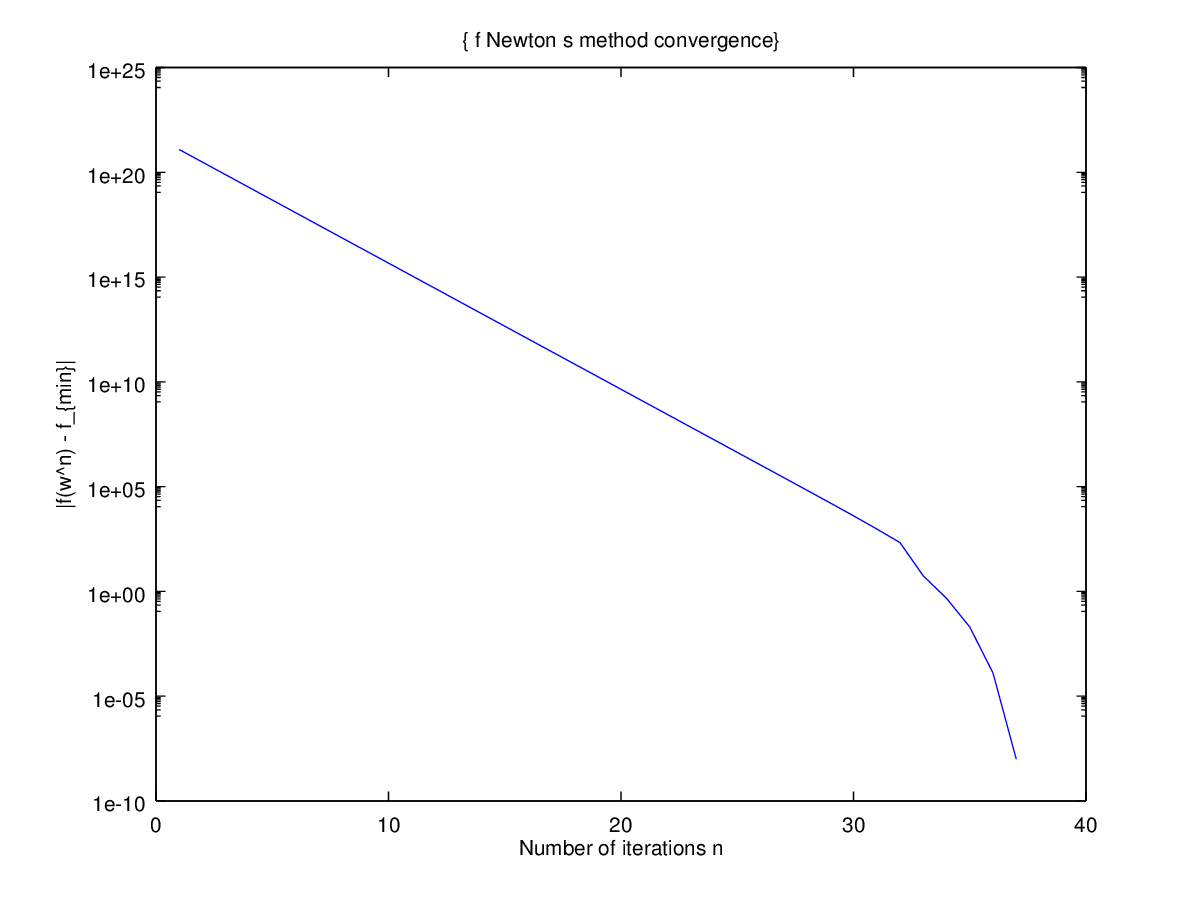
\includegraphics[scale=0.5]{images/cvnewton3.png}
             \caption{Ensemble de données 3 (échelle semi-log)}
           \end{center}
         \end{figure}

         \begin{figure}
           \begin{center}
             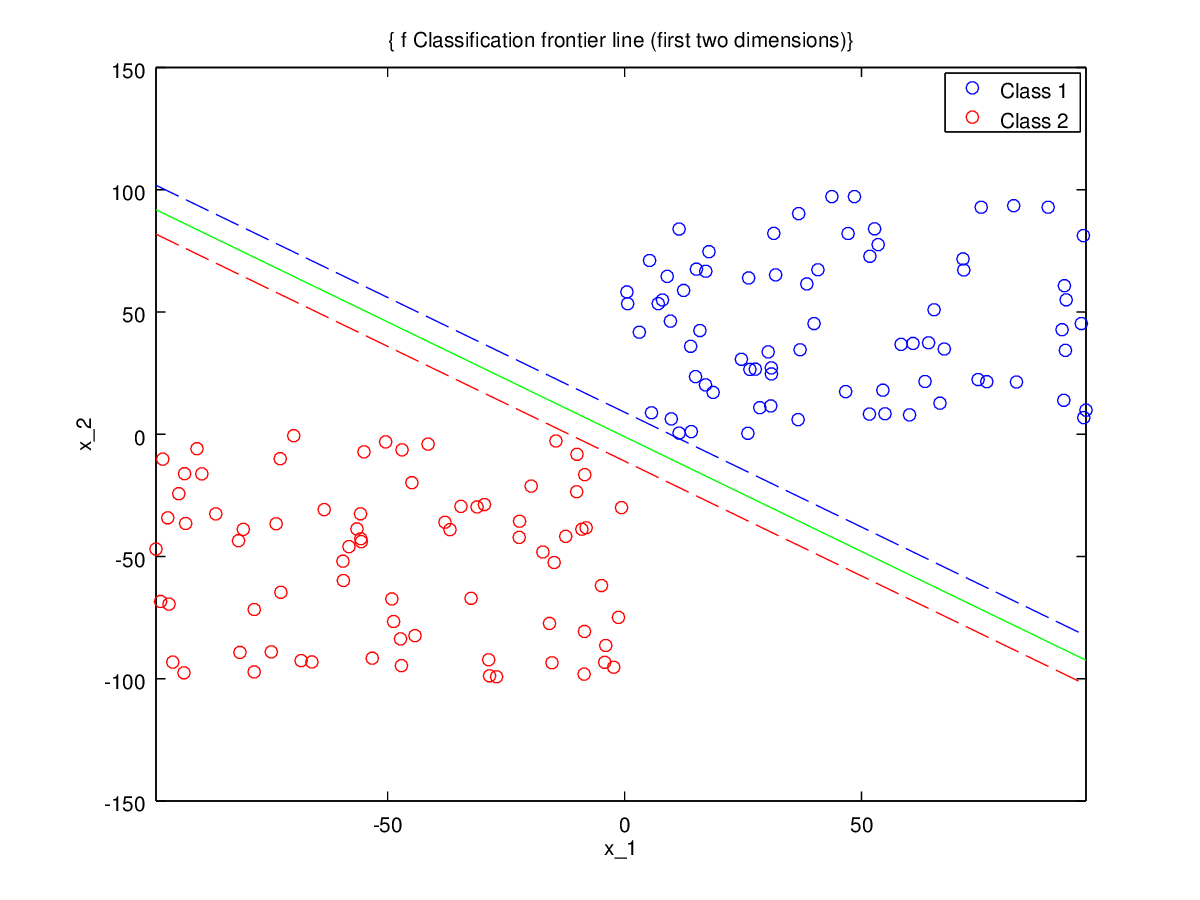
\includegraphics[scale=0.5]{images/line3.png}
             \caption{Ensemble de données 3 (Les lignes rouge et bleue en pointillés sont les droites f(x) = 10 et f(x) = -10)}
           \end{center}
         \end{figure}

         \begin{figure}
           \begin{center}
             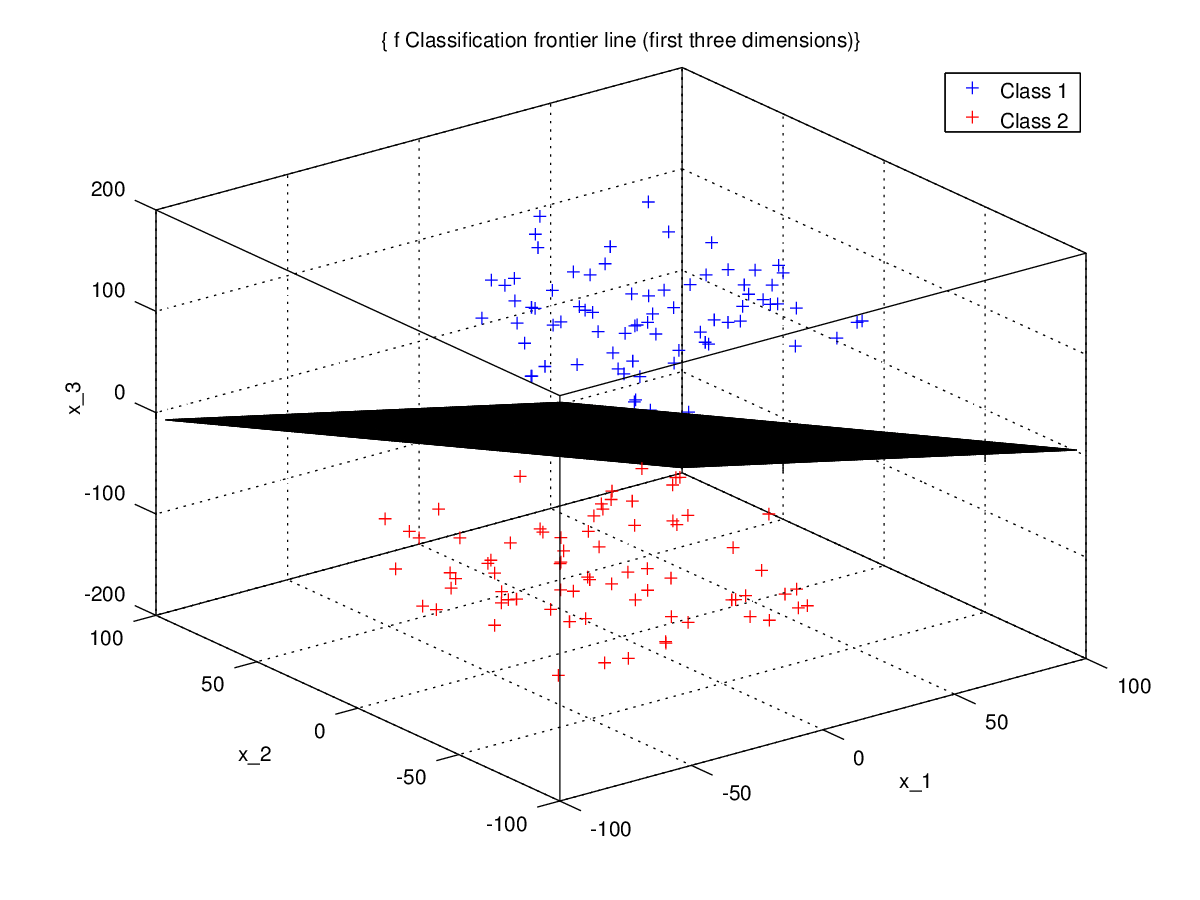
\includegraphics[scale=0.5]{images/plane3.png}
             \caption{Ensemble de données 3}
           \end{center}
         \end{figure}

         \begin{figure}
           \begin{center}
             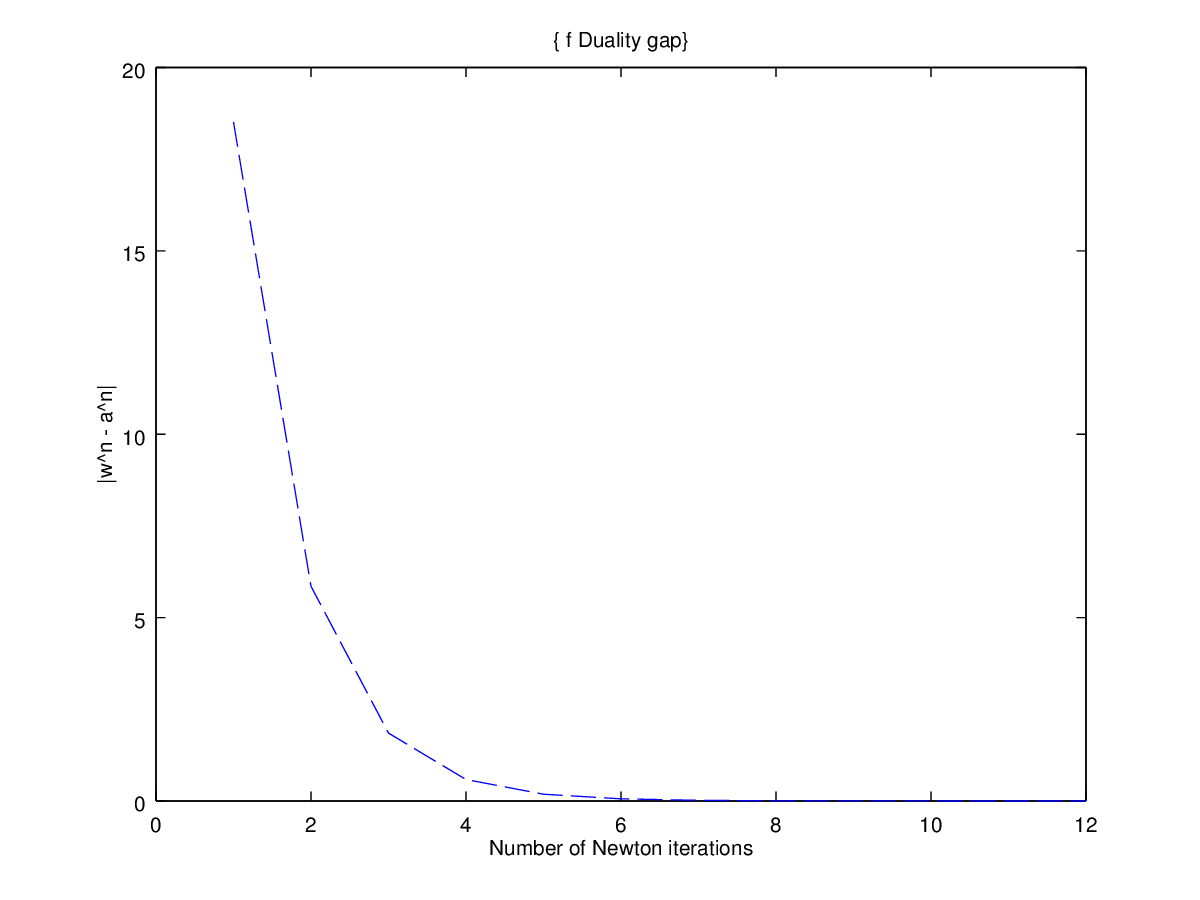
\includegraphics[scale=0.5]{images/duality3.png}
             \caption{\emph{Duality gap} : ensemble de données 3}
           \end{center}
         \end{figure}


\subsection{Points centrés réduits générés avec des fonctions gaussiennes}

On utilise la procédure $m=0$ dans \emph{generatedata.m} avec $sep=0$. Voir le fichier \emph{test4.mat} dans le dossier \emph{test}. 

\subsubsection{Pour $C=5, n=150, d=200$}

     \begin{table}[H]
       \caption{Matrice de confusion pour l'ensemble de données 4}
       \begin{tabular}{|l|c|r|}
         \hline
         \textsc{Réalité/Prédiction} & \textsc{Classe 1} & \textsc{Classe 2}\\
         \hline
         \textsc{Classe 1} & 28 & 0\\
         \hline
         \textsc{Classe 2} & 0 & 22\\
         \hline
       \end{tabular}
     \end{table}

         \begin{figure}
           \begin{center}
             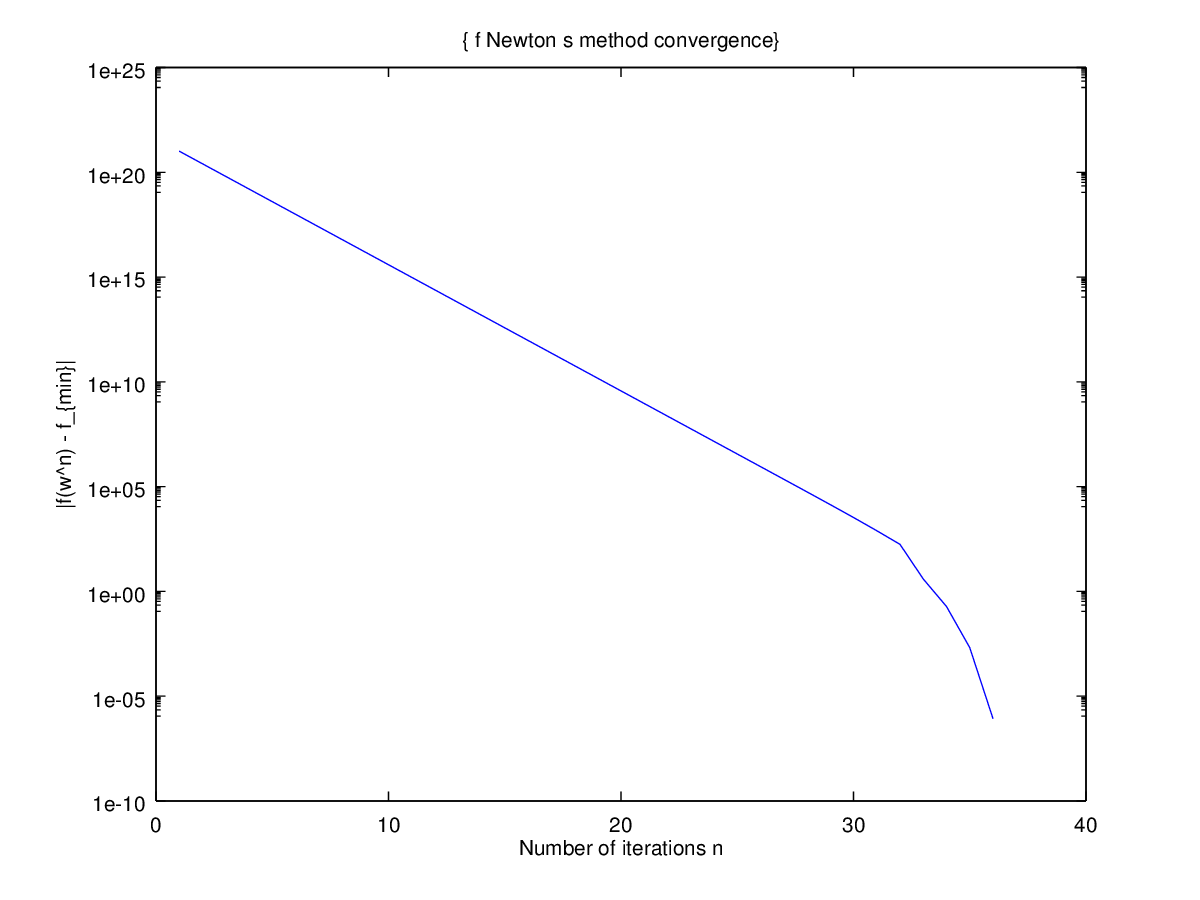
\includegraphics[scale=0.5]{images/cvnewton4.png}
             \caption{Ensemble de données 4 (échelle semi-log)}
           \end{center}
         \end{figure}

         \begin{figure}
           \begin{center}
             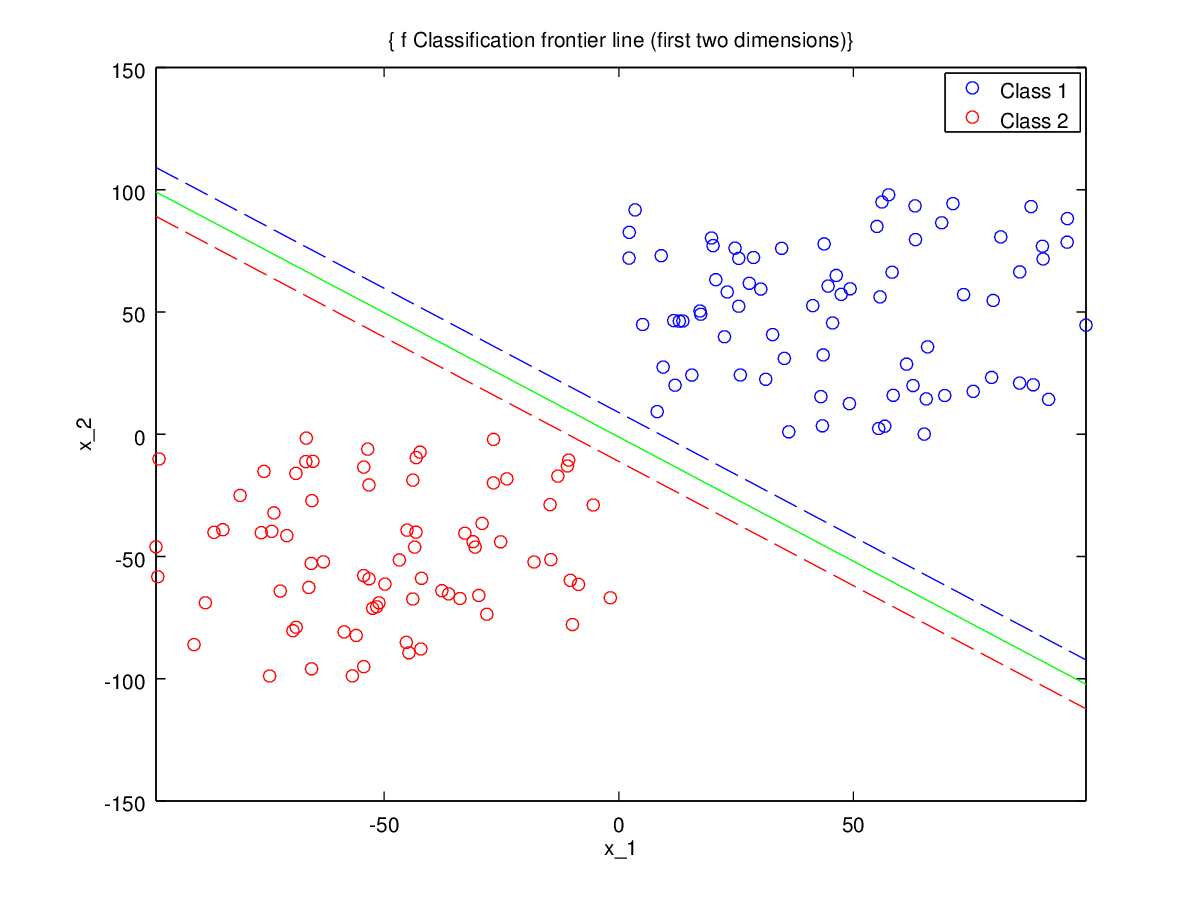
\includegraphics[scale=0.5]{images/line4.png}
             \caption{Ensemble de données 4 (Les lignes rouge et bleue en pointillés sont les droites f(x) = 10 et f(x) = -10)}
           \end{center}
         \end{figure}

         \begin{figure}
           \begin{center}
             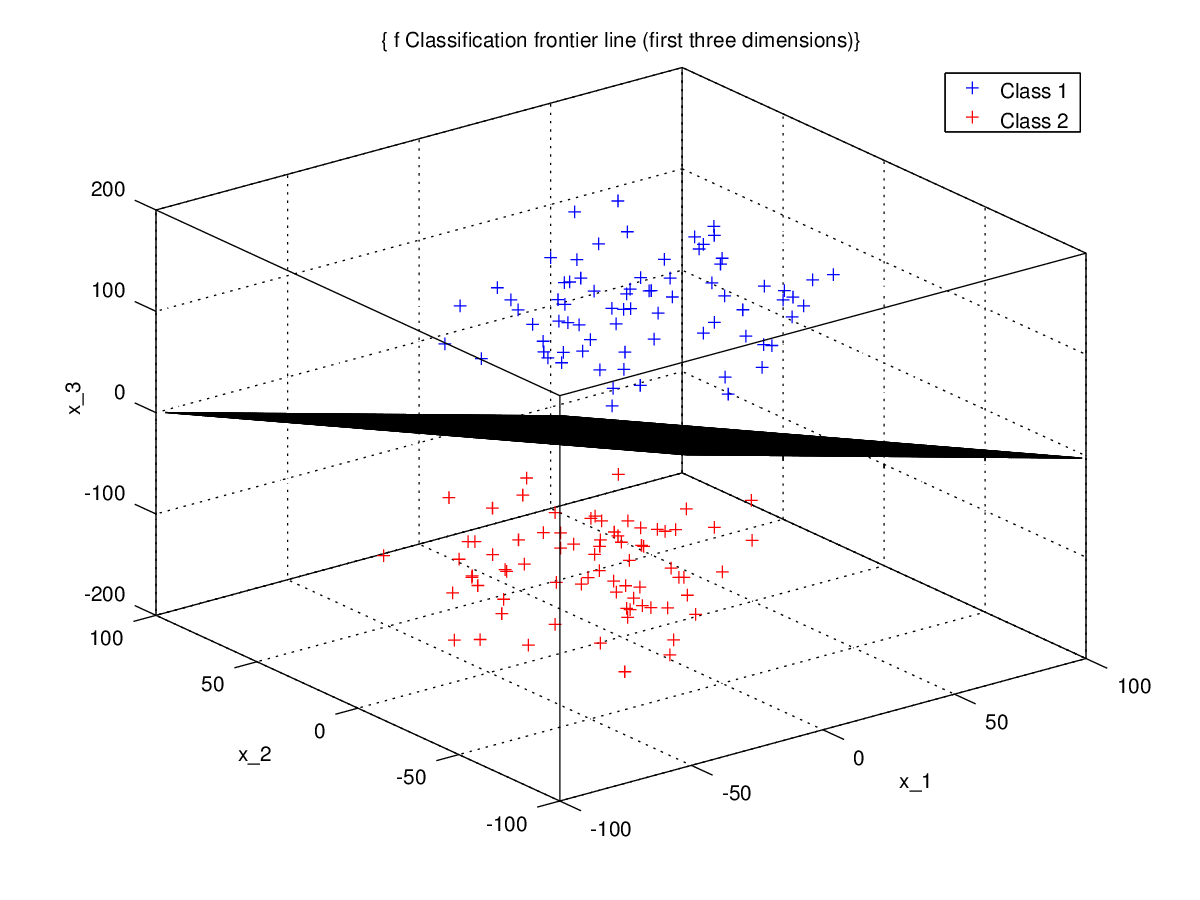
\includegraphics[scale=0.5]{images/plane4.png}
             \caption{Ensemble de données 4}
           \end{center}
         \end{figure}

         \begin{figure}
           \begin{center}
             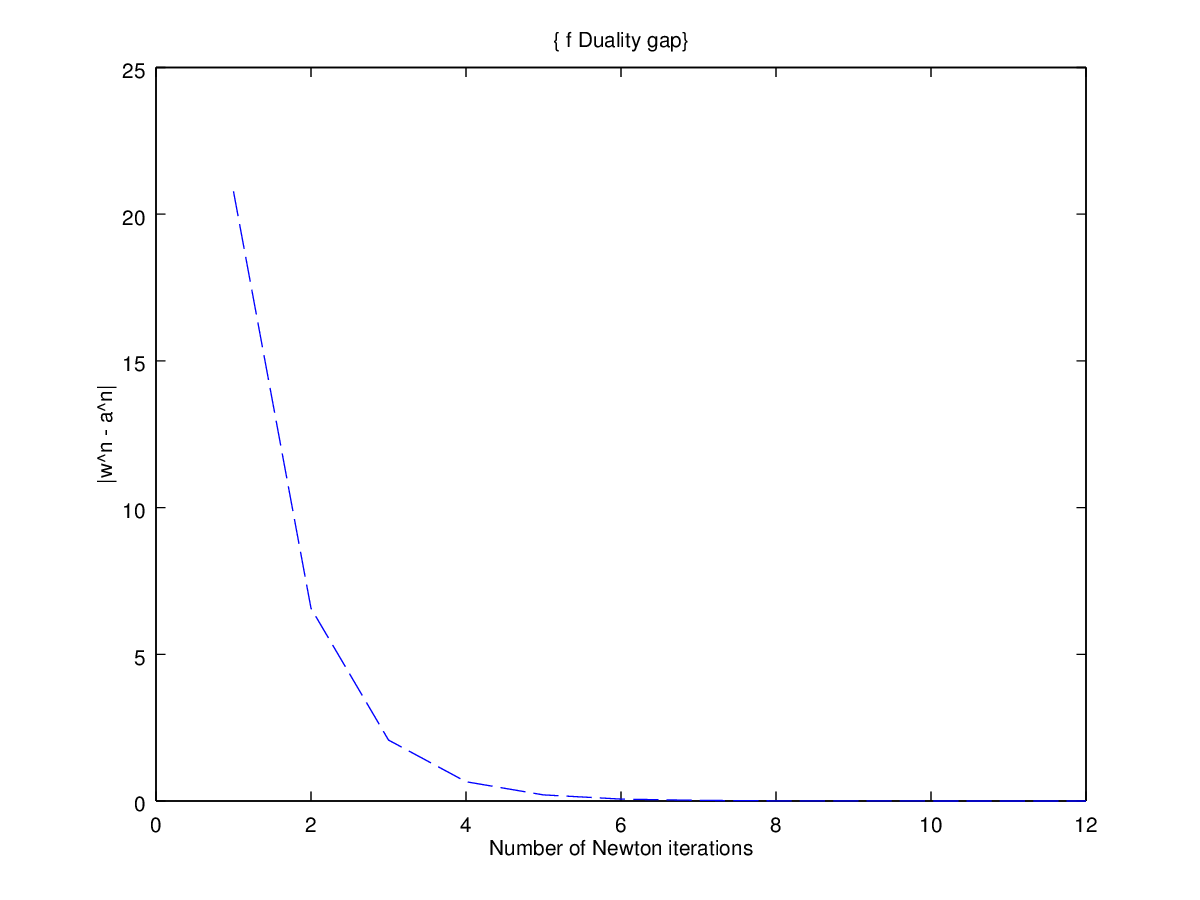
\includegraphics[scale=0.5]{images/duality4.png}
             \caption{\emph{Duality gap} : ensemble de données 4}
           \end{center}
         \end{figure}

\subsection{Points générés avec des fonctions gaussiennes}

On utilise la procédure $m=1$ dans \emph{generatedata.m} avec les paramètres par défaut. Voir le fichier \emph{test5.mat} dans le dossier \emph{test}.

\subsubsection{Pour $C=5, n=150, d=200$}

     \begin{table}[H]
       \caption{Matrice de confusion pour l'ensemble de données 5}
       \begin{tabular}{|l|c|r|}
         \hline
         \textsc{Réalité/Prédiction} & \textsc{Classe 1} & \textsc{Classe 2}\\
         \hline
         \textsc{Classe 1} & 9 & 1\\
         \hline
         \textsc{Classe 2} & 17 & 23\\
         \hline
       \end{tabular}
     \end{table}

         \begin{figure}
           \begin{center}
             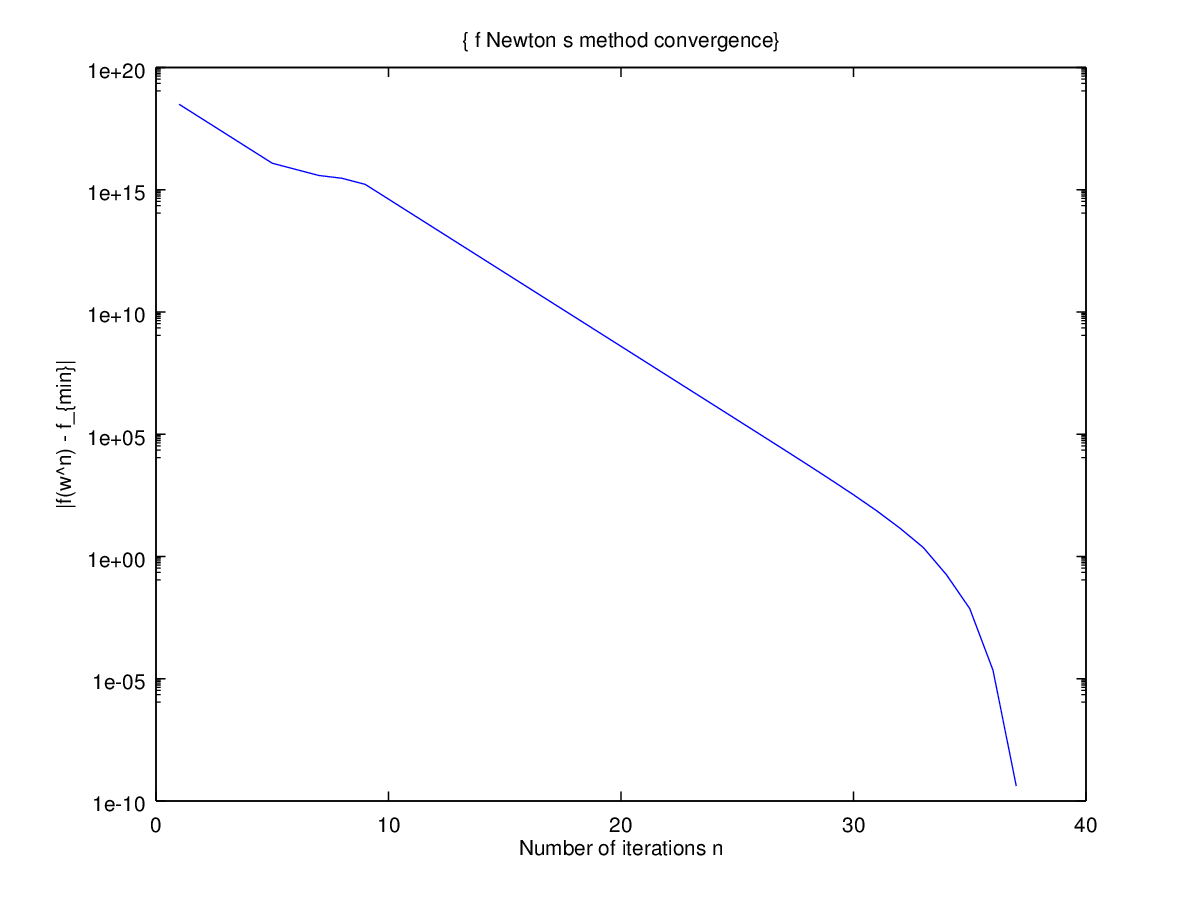
\includegraphics[scale=0.5]{images/cvnewton5.png}
             \caption{Ensemble de données 5 (échelle semi-log)}
           \end{center}
         \end{figure}

         \begin{figure}
           \begin{center}
             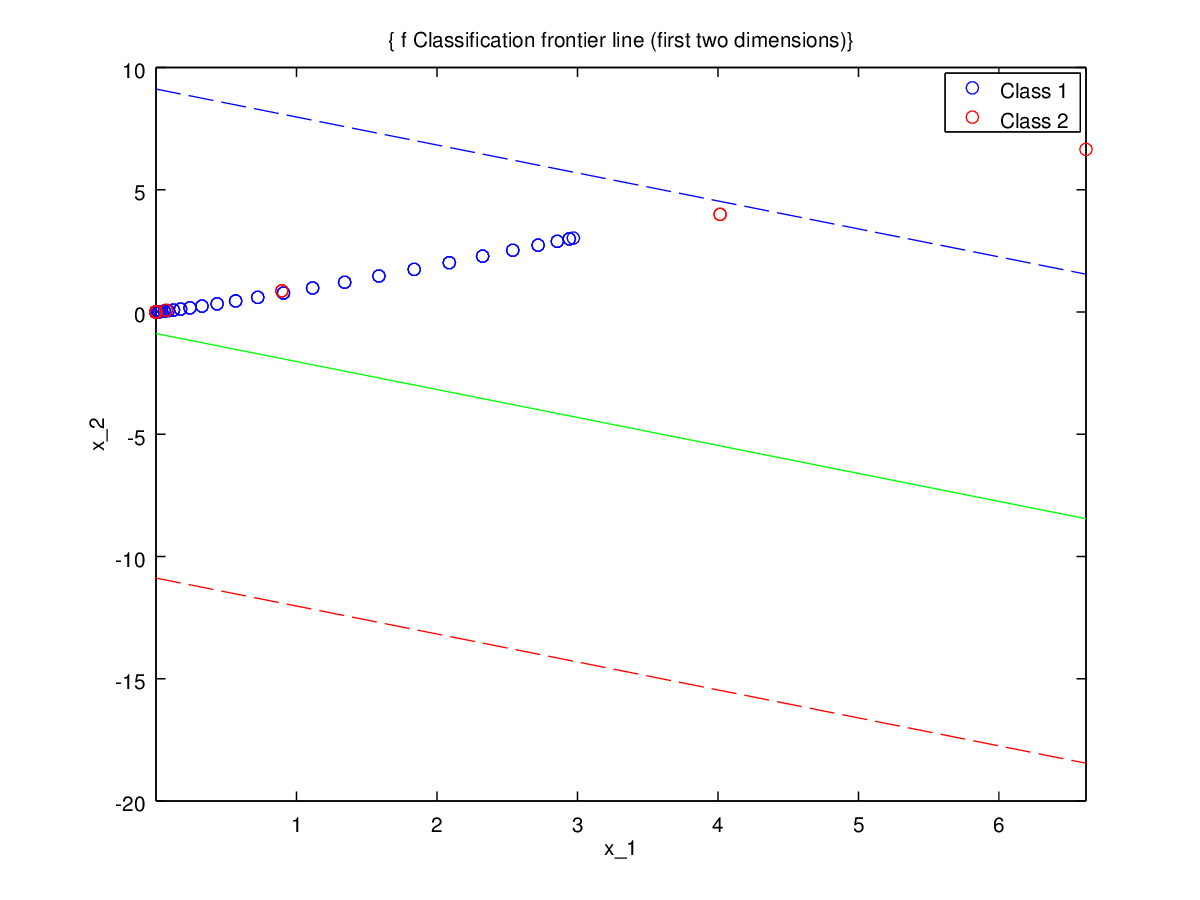
\includegraphics[scale=0.5]{images/line5.png}
             \caption{Ensemble de données 5 (Les lignes rouge et bleue en pointillés sont les droites f(x) = 10 et f(x) = -10)}
           \end{center}
         \end{figure}

         \begin{figure}
           \begin{center}
             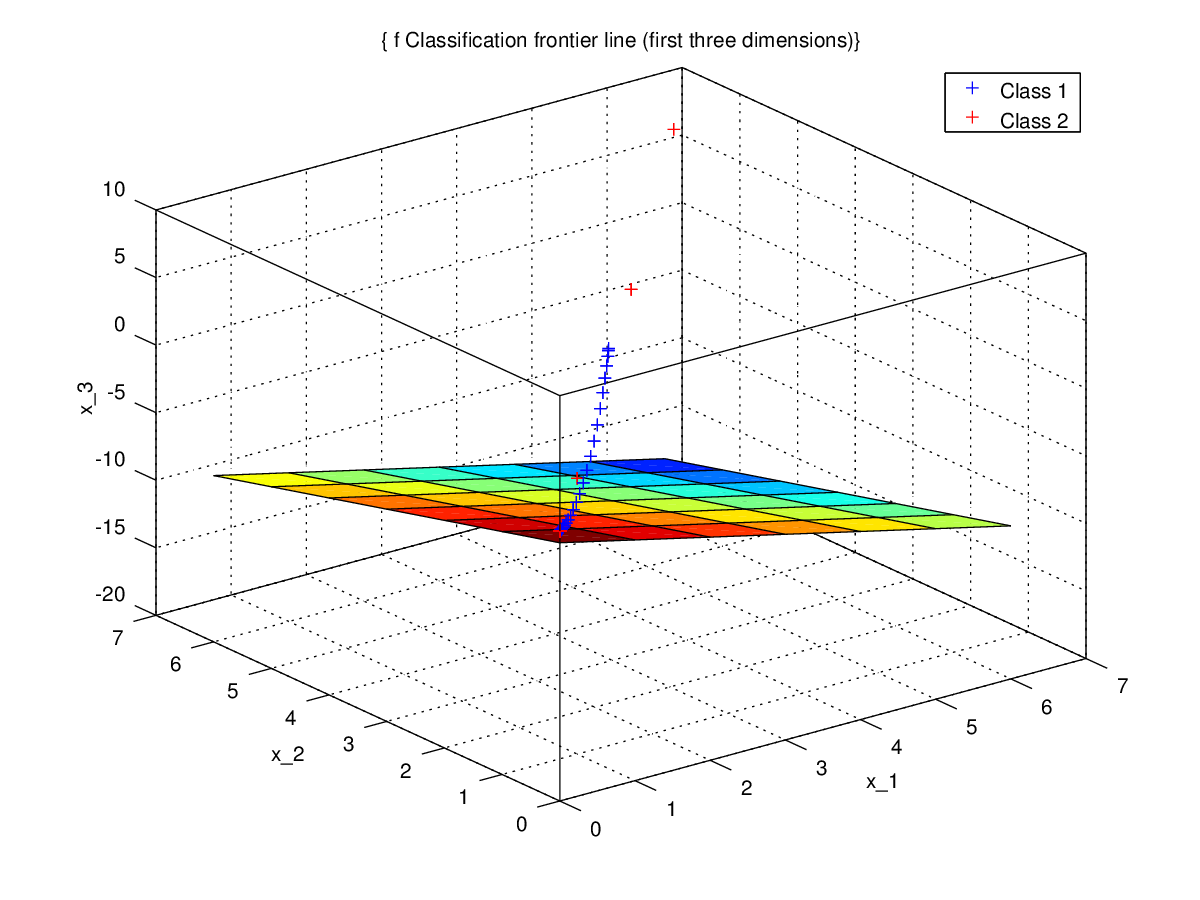
\includegraphics[scale=0.5]{images/plane5.png}
             \caption{Ensemble de données 5}
           \end{center}
         \end{figure}

         \begin{figure}
           \begin{center}
             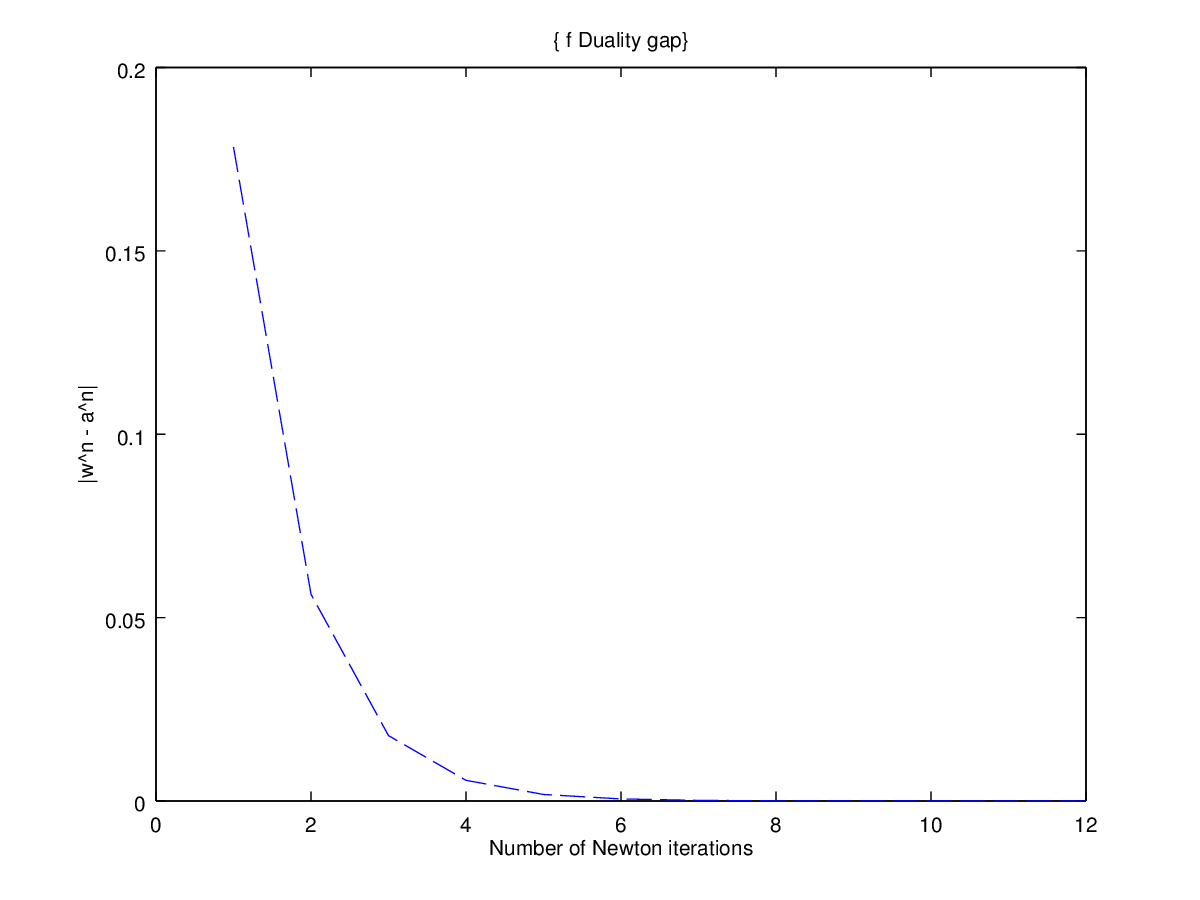
\includegraphics[scale=0.5]{images/duality5.png}
             \caption{\emph{Duality gap} : ensemble de données 5}
           \end{center}
         \end{figure}

\section{Comparaison avec \emph{la descente de coordonnées}}

\subsection{Résultats des ensembles de données précédents avec cette méthode}

$d$ est la dimension des points et $n$ le nombre d'échantillons dans la génération. On utilise $\frac{2}{3}$ des points (choisis au hasard uniformément) de l'ensemble de départ pour l'ensemble d'entraînement, et les points restants pour l'ensemble de validation. On considère les mêmes ensembles que précédemment (l'ensemble 1 est celui utilisé dans les trois premiers tests de la section précédente).\\

     \begin{table}[H]
       \caption{Comparaison entre les générations de points}
       \begin{tabular}{|l|c|c|c|c|r|}
         \hline
         \textsc{Données} & \textsc{C} & \textsc{d} & \textsc{n} & \textsc{Temps (s)} & \textsc{Echec (\%)}\\
         \hline
         1 & 1 & 40 & 10 & 0,021 & 0\\
         \hline
         1 & 5 & 40 & 10 & 0,015 & 0\\
         \hline
         1 & 10 & 40 & 10 & 0,012 & 0\\
         \hline
         3 & 1 & 200 & 150 & 0,322 & 0\\
         \hline
         5 & 1 & 200 & 150 & 0,392 & 54\\
         \hline
       \end{tabular}
     \end{table}

On constate que l'algorithme est beaucoup plus rapide que le précédent, mais donne de mauvais résultats dans le cas où les points sont générés à l'aide de deux fonctions gaussiennes. %DIRE POURQUOI

\subsection{Ensemble de données 1 ($C = 1$)}

     \begin{table}[H]
       \caption{Matrice de confusion pour l'ensemble de données 1}
       \begin{tabular}{|l|c|r|}
         \hline
         \textsc{Réalité/Prédiction} & \textsc{Classe 1} & \textsc{Classe 2}\\
         \hline
         \textsc{Classe 1} & 2 & 0\\
         \hline
         \textsc{Classe 2} & 0 & 1\\
         \hline
       \end{tabular}
     \end{table}

         \begin{figure}
           \begin{center}
             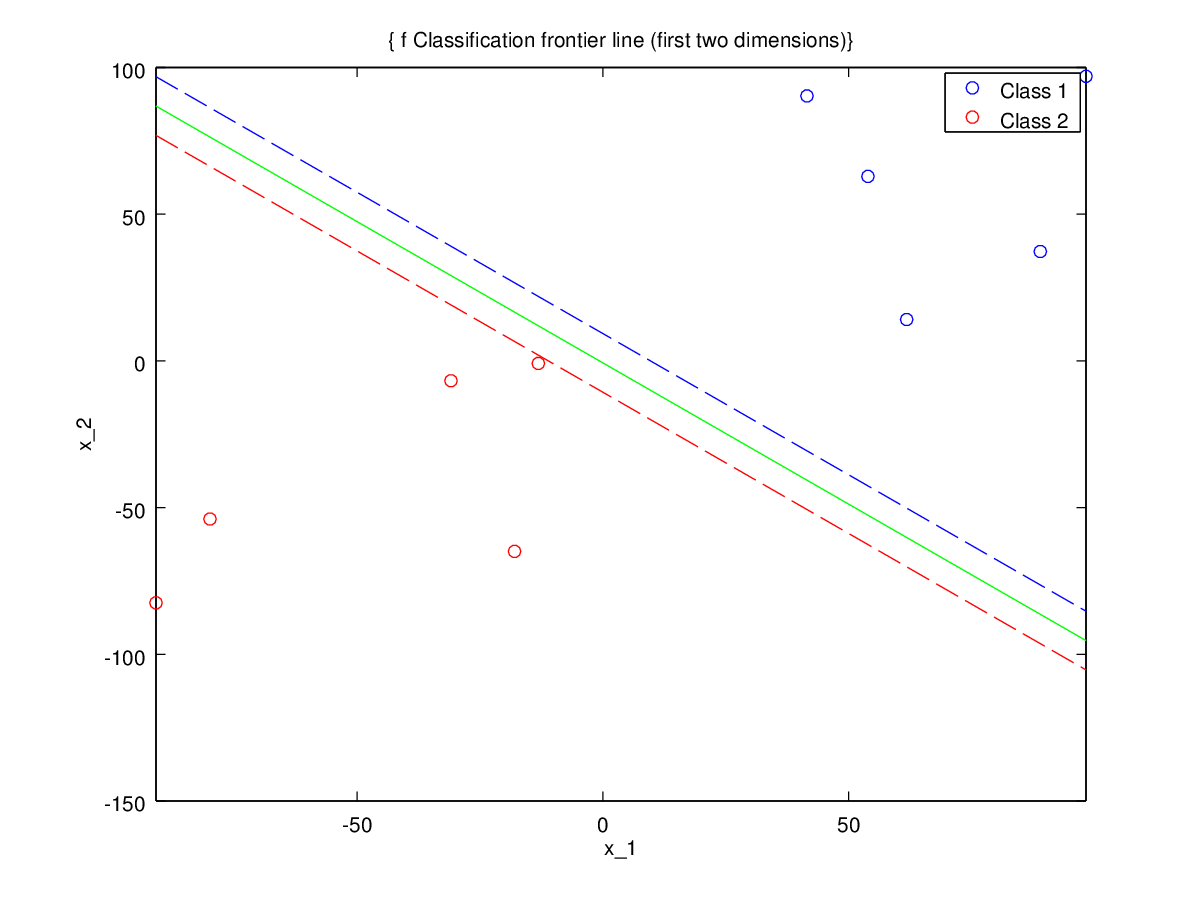
\includegraphics[scale=0.5]{images/line11.png}
             \caption{Ensemble de données 1 (Les lignes rouge et bleue en pointillés sont les droites f(x) = 10 et f(x) = -10)}
           \end{center}
         \end{figure}

         \begin{figure}
           \begin{center}
             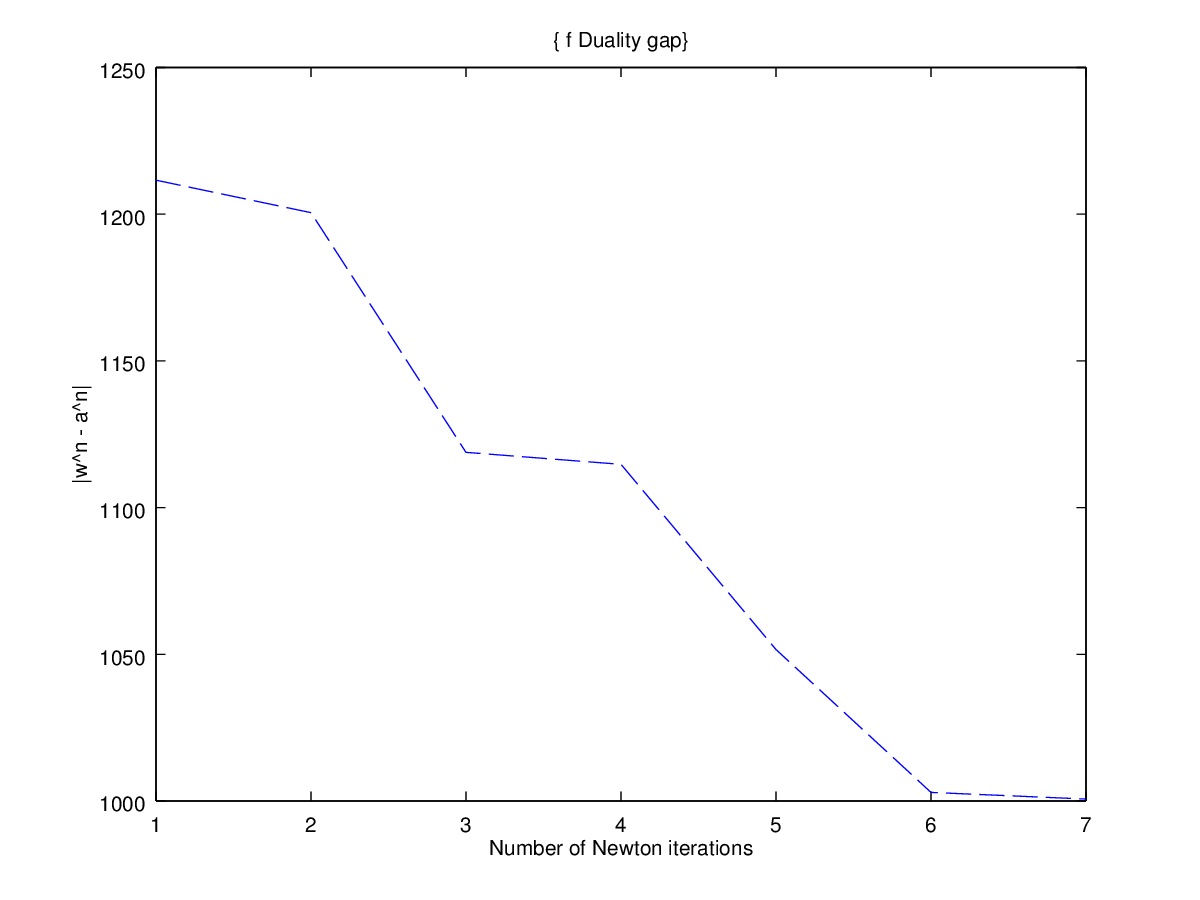
\includegraphics[scale=0.5]{images/duality11.png}
             \caption{\emph{Duality gap} : ensemble de données 1}
           \end{center}
         \end{figure}

\subsection{Ensemble de données 3}

     \begin{table}[H]
       \caption{Matrice de confusion pour l'ensemble de données 3}
       \begin{tabular}{|l|c|r|}
         \hline
         \textsc{Réalité/Prédiction} & \textsc{Classe 1} & \textsc{Classe 2}\\
         \hline
         \textsc{Classe 1} & 26 & 0\\
         \hline
         \textsc{Classe 2} & 0 & 24\\
         \hline
       \end{tabular}
     \end{table}

         \begin{figure}
           \begin{center}
             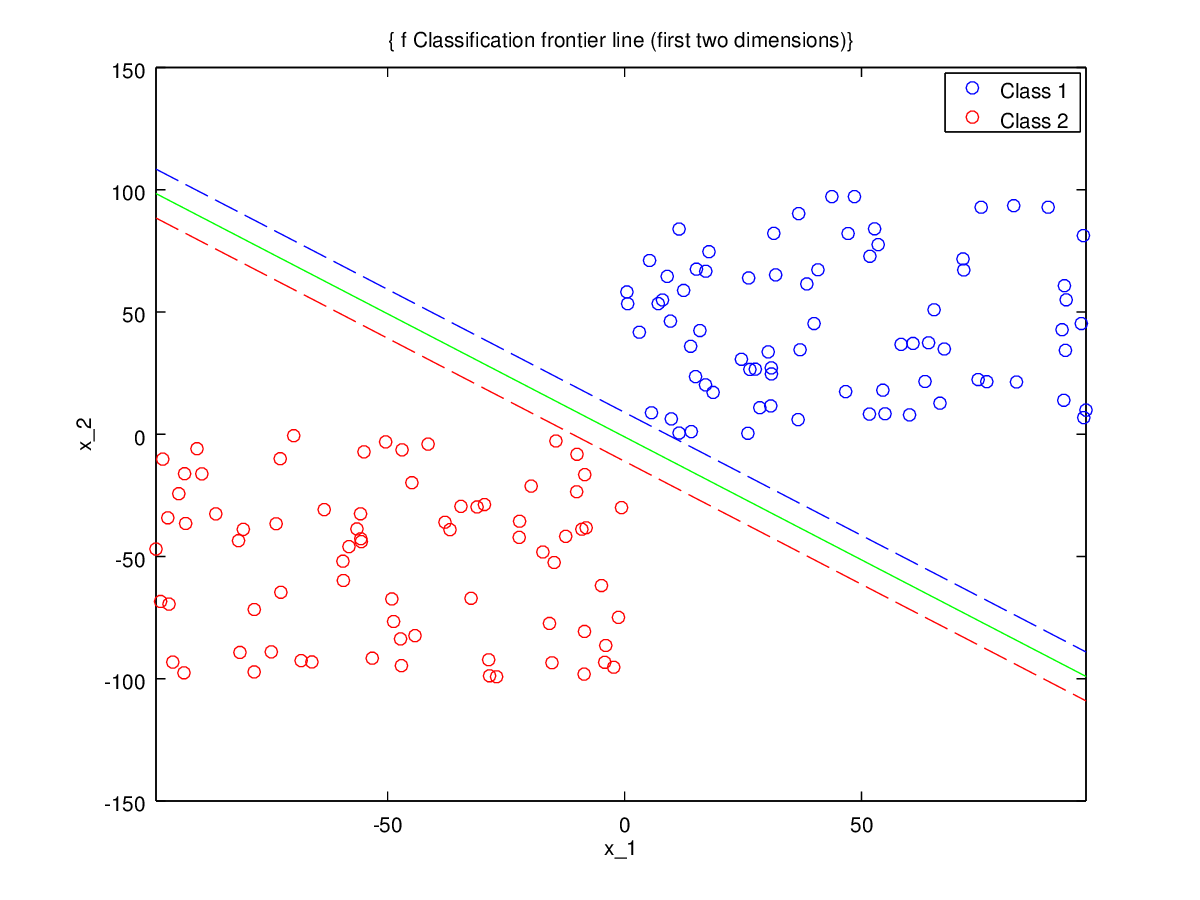
\includegraphics[scale=0.5]{images/line33.png}
             \caption{Ensemble de données 3 (Les lignes rouge et bleue en pointillés sont les droites f(x) = 10 et f(x) = -10)}
           \end{center}
         \end{figure}

         \begin{figure}
           \begin{center}
             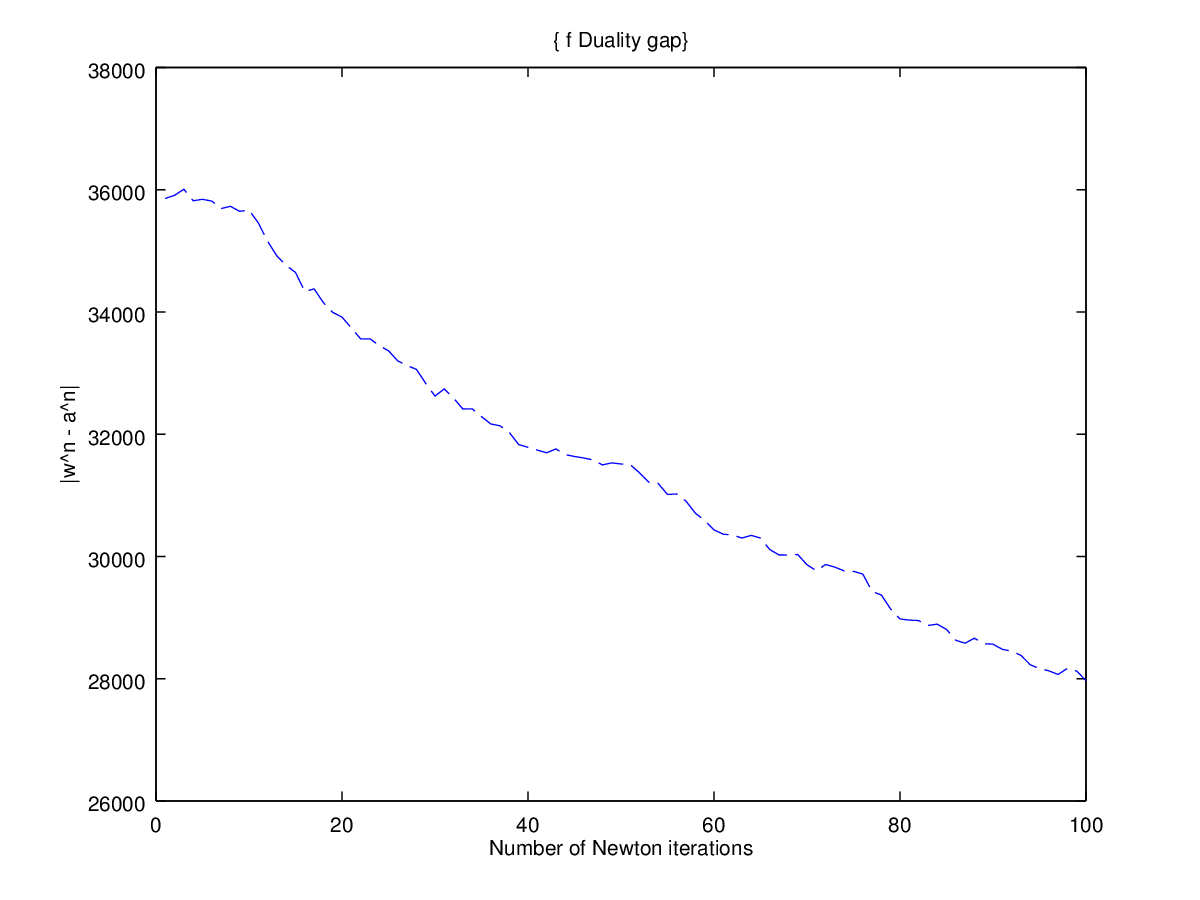
\includegraphics[scale=0.5]{images/duality33.png}
             \caption{\emph{Duality gap} : ensemble de données 3}
           \end{center}
         \end{figure}

\subsection{Ensemble de données 5}

     \begin{table}[H]
       \caption{Matrice de confusion pour l'ensemble de données 5}
       \begin{tabular}{|l|c|r|}
         \hline
         \textsc{Réalité/Prédiction} & \textsc{Classe 1} & \textsc{Classe 2}\\
         \hline
         \textsc{Classe 1} & 21 & 20\\
         \hline
         \textsc{Classe 2} & 7 & 2\\
         \hline
       \end{tabular}
     \end{table}

         \begin{figure}
           \begin{center}
             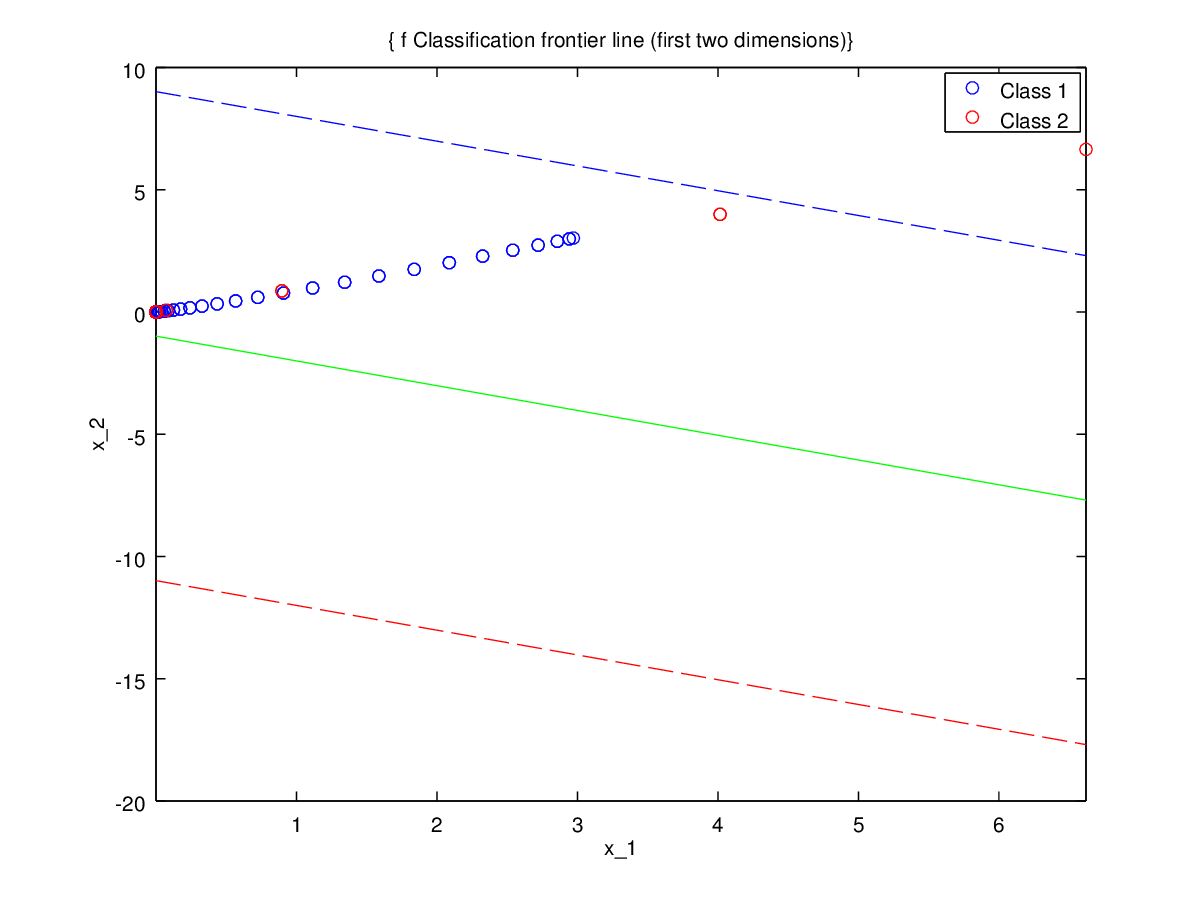
\includegraphics[scale=0.5]{images/line55.png}
             \caption{Ensemble de données 5 (Les lignes rouge et bleue en pointillés sont les droites f(x) = 10 et f(x) = -10)}
           \end{center}
         \end{figure}

         \begin{figure}
           \begin{center}
             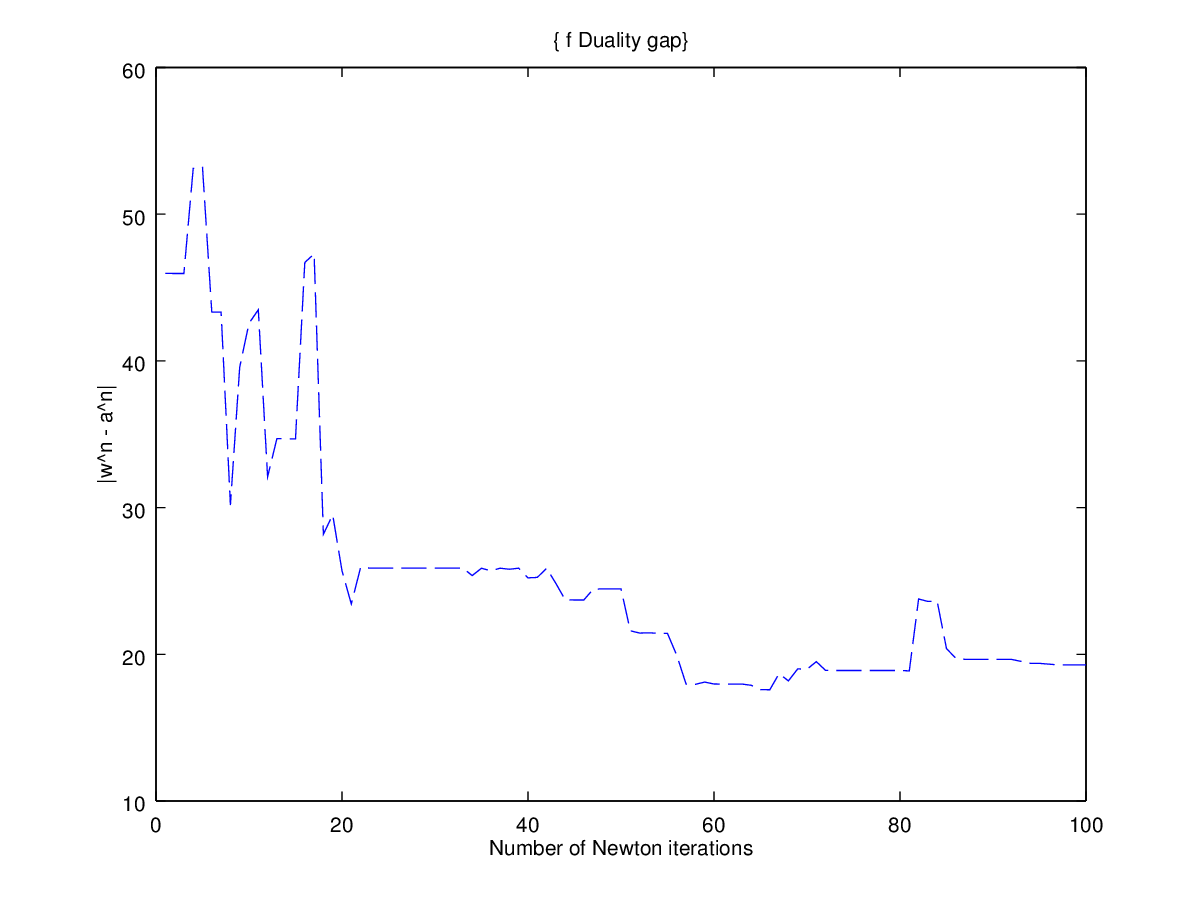
\includegraphics[scale=0.5]{images/duality55.png}
             \caption{\emph{Duality gap} : ensemble de données 5}
           \end{center}
         \end{figure}

% COMMENTER

\end{document}
